\documentclass[paper=a4,11pt,parskip=half,toc=listof]{scrartcl}
\usepackage{etoolbox}
\newtoggle{german}

% % % % % LANGUAGE % % % %
% Make your choice here
\togglefalse{german} % English
%\toggletrue{german} % German
% % % % % \LANGUAGE % % % %

\iftoggle{german}{
\usepackage[ngerman]{babel} % Deutsche Sprachanpassungen
\usepackage[T1]{fontenc}    % Silbentrennung bei Sonderzeichen
\usepackage[utf8]{inputenc} % Direkte Angabe von Umlauten im Dokument.Wenn Sie an einem Mac sitzen,verwenden Sie ggf. „macce“ anstatt „utf8“.
\usepackage[autostyle=true,german=quotes]{csquotes} % Anfuehrungszeichen\
}{
\usepackage[utf8]{inputenc}}
\usepackage{enumitem}
\usepackage{scrpage2}
\usepackage{listings}
\usepackage{color}
\usepackage{textcomp}
\usepackage{mathtools}
\usepackage{nicefrac}
\usepackage{amsmath}
\usepackage[T1]{fontenc}
\usepackage[german]{translator}
\usepackage{pgfgantt}
\usepackage{graphicx}
\usepackage{longtable}
\usepackage{float}
\usepackage{setspace}
\usepackage{url}
\usepackage{tabularx}
\usepackage{makecell}
\usepackage{multirow}
\usepackage{wrapfig}
\usepackage{pdfpages}
\usepackage{amssymb}
\usepackage{graphicx}
\usepackage[font=small]{caption} % very thin
\usepackage{subcaption}
\usepackage{picinpar}
\usepackage{multicol}
\usepackage{tcolorbox}
\usepackage{rotating}

%Bibliography
\usepackage[
backend=biber,
style=ieee,
sortlocale=en_GB,
natbib=true,
url=false, 
doi=true,
isbn=true,
eprint=false
]{biblatex}


\addbibresource{references.bib}
% No footnotes on the next page please
\interfootnotelinepenalty=10000
\lstdefinelanguage{TypeScript}{
  keywords={typeof, new, true, false, catch, function, return, null, catch, switch, var, if, in, while, do, else, case, break, const, let, interface, type, extends},
  keywordstyle=\color{blue}\bfseries,
  ndkeywords={class, export, boolean, throw, implements, import, this},
  ndkeywordstyle=\color{darkgray}\bfseries,
  identifierstyle=\color{black}\ttfamily,
  sensitive=false,
  comment=[l]{//},
  morecomment=[s]{/*}{*/},
  commentstyle=\color{purple}\ttfamily,
  stringstyle=\color{red}\ttfamily,
  morestring=[b]',
  morestring=[b]",
  morestring=[b]`
}

\lstset{ 
  language=TypeScript,                 % the language of the code
  backgroundcolor=\color{white},   % choose the background color; you must add \usepackage{color} or \usepackage{xcolor}; should come as last argument
  basicstyle=\footnotesize,        % the size of the fonts that are used for the code
  breakatwhitespace=false,         % sets if automatic breaks should only happen at whitespace
  breaklines=true,                 % sets automatic line breaking
  captionpos=b,                    % sets the caption-position to bottom
  extendedchars=true,              % lets you use non-ASCII characters; for 8-bits encodings only, does not work with UTF-8
  frame=single,	                   % adds a frame around the code
  keepspaces=true,                 % keeps spaces in text, useful for keeping indentation of code (possibly needs columns=flexible)
  keywordstyle=\color{blue},       % keyword style
  numbers=left,                    % where to put the line-numbers; possible values are (none, left, right)
  numbersep=5pt,                   % how far the line-numbers are from the code
  numberstyle=\color{gray}\bfseries, % the style that is used for the line-numbers
  rulecolor=\color{black},         % if not set, the frame-color may be changed on line-breaks within not-black text (e.g. comments (green here))
  showspaces=false,                % show spaces everywhere adding particular underscores; it overrides 'showstringspaces'
  showstringspaces=false,          % underline spaces within strings only
  showtabs=false,                  % show tabs within strings adding particular underscores
  stepnumber=1,                    % the step between two line-numbers. If it's 1, each line will be numbered
  tabsize=2,	                   % sets default tabsize to 2 spaces
  title=\lstname                   % show the filename of files included with \lstinputlisting; also try caption instead of title
}
%opening

% Introduction of a design system to establish a frontend engineering and design platform
% Creation of a front-end platform by introducing a design system
% Introduction of a design system - A frontend engineering and design platform
\def\ThesisTitle{User interface standardization of \acl{SaaS} products}
\def\ThesisAuthor{Tom Gehder}
\def\ThesisLocation{Sankt Augustin}
\def\ThesisType{Master}
\def\CourseType{Computer Science}
\def\ThesisPubDate{\today} % Change here to the date you are going to print your thesis
\def\ThesisFirstSupervisor{Prof. Dr. Manfred Kaul}
\def\ThesisSecondSupervisor{Prof. Dr. Sascha Alda}
\def\ThesisExternalSupervisor{-}
\def\ThesisExternalCompany{LeanIX GmbH}
\def\ThesisSubject{}


\usepackage{todonotes}
\usepackage{pdfpages} % directly include pdf pages
\usepackage{algorithmic} % pseudo-code
\usepackage{blindtext}
\usepackage[printonlyused]{acronym} 
%\usepackage[firstpage]{draftwatermark} % comment in if you submit a draf. 
\DeclarePairedDelimiter{\ceil}{\lceil}{\rceil}

% new types for a table
\newcolumntype{C}[1]{>{\centering\arraybackslash}p{#1}}
\newcommand{\specialcell}[2][l]{%
  \begin{tabular}[#1]{@{}c@{}}#2\end{tabular}}
  



%%%% Font %%%%
% \usepackage{times} % times in text
\usepackage{mathptmx} % times in math
\usepackage{setspace} \onehalfspacing %
\usepackage[paper=a4paper]{geometry}
\setlength{\parindent}{0pt} % no indent
\setlength{\headheight}{1.1\baselineskip}
\setcounter{tocdepth}{4}
\setcounter{secnumdepth}{4}
%%%% Font %%%%

%%%% footer and header %%%%
\usepackage{scrpage2}%
\pagestyle{scrheadings}%  S
\clearscrheadfoot% 
\setheadwidth{text}%
\automark{section}% 
\ohead{\textbf{\pagemark}}
\renewcommand{\sectionmark}[1]{\markright{\ #1}} 
\ihead{\textbf{\rightmark}}
\setheadsepline{0.5pt}
%%%% \footer and header %%%%

\newcolumntype{Y}{>{\centering\arraybackslash}X}




\usepackage{hyperref}
\hypersetup{
    unicode=false,          % non-Latin characters in Acrobat’s bookmarks
    pdftoolbar=true,        % show Acrobat’s toolbar?
    pdfmenubar=true,        % show Acrobat’s menu?
    pdffitwindow=false,     % window fit to page when opened
    pdfstartview={FitH},    % fits the width of the page to the window
    pdftitle={\ThesisTitle},    % title
    pdfauthor={\ThesisAuthor},     % author
    pdfsubject={\ThesisTitle},   % subject of the document
    pdfcreator={\ThesisAuthor},   % creator of the document
    pdfproducer={\ThesisAuthor}, % producer of the document
    pdfkeywords={802.11} {DCF} {long-distance} {modeling}, % list of keywords
    pdfnewwindow=true,      % links in new window
    colorlinks=false,       % false: boxed links; true: colored links
    linkcolor=red,          % color of internal links (change box color with linkbordercolor)
    citecolor=green,        % color of links to bibliography
    filecolor=magenta,      % color of file links
    urlcolor=cyan           % color of external links
}


\begin{document}
%%%%%%%%%%%%%%%%%%%%% Startseite %%%%%%%%%%%%%%%%%%%%%%%%%%%
\begin{titlepage}
\begin{minipage}[t]{1\textwidth}
\begin{Large}
    \begin{flushleft}
      \hspace{1cm} \makebox[2cm][c]{
\includegraphics[height=8ex]{./logos/logo_hbrs.png} \vspace{1.8cm}}
%      \hspace{1cm} \makebox[10cm][r]{
\includegraphics[height=8ex]{./logos/logo_leanix.png} \vspace{1.8cm}}
    \end{flushleft}
\end{Large}
\end{minipage}
%\begin{minipage}[t]{0.5\textwidth}
% Can be an external company! Play with thge vspaces to look nice.
%\begin{Large}
%    \begin{flushright}
%     \makebox[3cm][c]{
\includegraphics[height=8ex]{./logos/logo_hbrs.png} \vspace{1.8cm}} \hspace{1cm}
%    \end{flushright}
%\end{Large}
%\end{minipage}
\vspace{0.07\textheight}
\iftoggle{german}{%
\begin{center}
\begin{Huge}
\textbf{Exposé}\\
\end{Huge}
\vspace{0.07\textheight}
\begin{Large}
Masterprojekt \\
\end{Large}
\begin{Large}
im Studiengang \\
\CourseType \\
\end{Large}
\end{center}
}{
\begin{center}
\begin{Huge}
\textbf{Master Thesis} \\
\vspace{0.07\textheight}
\begin{Large}
\CourseType \\
\end{Large}
\end{Huge}
\end{center}
}
\vspace{0.03\textheight}
\begin{center}
 \begin{Huge} \begin{spacing}{1.3} \textbf{\ThesisTitle} \end{spacing} \end{Huge}
 \vspace{2em}
 \iftoggle{german}{%
  \begin{Large}\textbf{von} \end{Large}\\
 }
 {%
  \begin{Large}\textbf{by} \end{Large}\\
 }
 \vspace{2em}
 \begin{Large}\textbf{\ThesisAuthor}\end{Large}\\
\end{center}
%\vspace{0.100\textheight}
\begin{large}
\begin{flushleft}
% use packages: array
\vfill
\iftoggle{german}{%
\begin{tabularx}{\textwidth}{lX}
 Erstprüfer: & \ThesisFirstSupervisor \\
 Zweitprüfer: & \ThesisSecondSupervisor \\
 Betreuer: & \ThesisExternalSupervisor \\
 Unternehmen:  & \ThesisExternalCompany \\ % Comment out if not needed
 Eingereicht am: & \ThesisPubDate % Comment out if not needed
\end{tabularx}
}
{%
\begin{tabularx}{\textwidth}{lX}
 First supervisor: & \ThesisFirstSupervisor \\
 Second supervisor: & \ThesisSecondSupervisor \\
 External supervisor: & \ThesisExternalSupervisor \\
 External company: ~ & \ThesisExternalCompany \\ % Comment out if not needed
 Handed in: & \ThesisPubDate % Comment out if not needed
\end{tabularx}
}




\end{flushleft}
\end{large}
\end{titlepage}

\newgeometry{top=4cm, bottom=3cm, left=4.5cm, right=3cm}
Name: Tom Gehder \\
Adresse: Weberstraße 79, 53113 Bonn\\

\section*{Erklärung}
Hiermit erkläre ich an Eides Statt, dass ich die vorliegende Arbeit selbst angefertigt
habe; die aus fremden Quellen direkt oder indirekt übernommenen Gedanken sind
als solche kenntlich gemacht.\\

Die Arbeit wurde bisher keiner Prüfungsbehörde vorgelegt und auch noch nicht
veröffentlicht.


\begin{table}[b]
    \begin{tabular}{p{0.5\linewidth} p{0.5\linewidth}}
        Unterschrift & Sankt Augustin, den \\
        \hline
    \end{tabular}
\end{table}

\pagenumbering{Roman} % Big roman numbers
\addtocontents{toc}{\protect\markright{}}

\newpage
\tableofcontents
\cleardoublepage
\pagenumbering{arabic}
\newpage
\listoftables % add list of tables
\listoffigures % add list of figures 
\lstlistoflistings % add list of listings 
\section*{List of Abbreviations}
\begin{acronym}
    \acro{SDS}[SDS]{SaaS Design System}
    \acro{SaaS}[SaaS]{Software as a Service}
    \acro{UX}[UX]{User-Experience}
    \acro{UI}[UI]{User Interface}
    \acro{CSS}[CSS]{Cascading Style Sheets}
    \acro{HTML}[HTML]{Hypertext Markup Language}
    \acro{DOM}[DOM]{Document Object Model}
    \acro{ES6}[ES6]{ECMAScript 6}
    \acro{SCSS}[SCSS]{Sassy CSS}
    \acro{NPM}[NPM]{Node Package Manager}
    \acro{RFC}[RFC]{Request for Comments}
    \acro{API}[API]{application interface}

\end{acronym} % include the acronym thing

\setcounter{page}{1}
\newpage
%%%%%%%%%%%%%%%%%%%%% Startseite %%%%%%%%%%%%%%%%%%%%%%%%%%%
\setcounter{tocdepth}{4} 
\setcounter{secnumdepth}{4}

\pagenumbering{arabic} % arabic numbers for the main part

% Here the chapters are included

\section{Introduction}
Standardization in technology is an important topic of great significance. Without standardization, there would be no progress in computer science today. \\
A look at the past shows that the first attempt at standardization was made in the 18th century. During the industrial revolution, standards were urgently needed to align and reliably connect machines. Thus, the first known standard was created with the screw and nut. Building on this, technology was able to spread and develop rapidly during this time. \cite{wiki_standardization_2022} \\
Today, no one thinks about the specification of a bolt or a nut when they use it. That is the goal of standardization. Forget about things that have already been thought about. Topics can move much faster if people can  focus on the relevant work. \\

\subsection{\acl{SaaS}}

In a world of technology, a new star has risen in recent years, namely \acl{SaaS}. \acl{SaaS} is a discipline of cloud computing. The cloud generally hosts \ac{SaaS} applications with which users can interact via the Internet. In this way, providing users with services that previously required them to install software on their desktops is much easier. In addition, this type of software often comes with a subscription model that allows users to switch from one software to another within a month. \\
\ac{SaaS} providers take care of all infrastructure issues, so the end user doesn’t have to worry about those issues. In return, the end user pays for the full service, not just the actual application. \\
Since this type of software is available over the Internet, any connected device can access the software through a web browser. The buzzword Web 2.0 describes the evolution away from on-premise software to services delivered online. The web browser is the primary interaction tool when working with \ac{SaaS} products. Most of the products build their user interfaces web-based. \cite{hill_guide_2013}\\
\citeauthor{hill_guide_2013} summarizes the characteristics of \ac{SaaS} software as follows:
\begin{itemize}
    \item Software that is available worldwide via the Internet free of charge or for a fee
    \item Collaborative
    \item Automatic update of the software products by the manufacturer
    \item All users use the same version of the application
    \item Software product automatically scales as needed
    \item Central management reduces the cost of distribution and maintenance in the 
    cloud
\end{itemize}
The popularity of \ac{SaaS} products is steadily increasing. Not only is it easy for the end user to use such software without having to install anything on his computer, but \ac{SaaS} products are also becoming more and more attractive for smaller companies. Often, the number of product users is the base for the payment plans. Therefore, even small businesses can afford software, which was not possible before. \cite{sury_software-as--service-modell_2020}\\
The number of \ac{SaaS} products used in companies has increased tenfold in the last five years. \cite{stastista_saas_2021} The need for standardization to align software is pressing at this high rate. Naturally, when thinking about alignment, a software architect thinks about connecting systems via application interfaces. These interfaces are often well documented and offer a variety of options. But what about maybe the most critical interface of the software, the user interface?
\subsection{User interfaces in \ac{SaaS} products}
Users are still the primary consumers of \ac{SaaS} products. And that will not change in the next ten years. More and more SaaS products will emerge, and one will be replaced by the other. Depending on what works best for the current use case. The products used in businesses could change from month to month. For users, this means they will have to learn new structures and workflows of each software from scratch again. Of course, there may be tutorials, training, and documentation. But in real life, users learn how to use the software when working with it. \\
An excellent example of this is a blog post by \citeauthor{sernoff_website_2021} that shows how many different implementations of a navigation menu exist. No wonder the sheer amount of variants can confuse users. It may take some time for a user to remember each interaction pattern for each software. And this example refers only to navigation menus.  Usually, user interfaces consist of many different components, which leads to even more confusion when switching between various programs. \\
Therefore, software programs must have similar user interfaces. For comparison: The arrangement of the pedals in motorized vehicles is always the same. Car manufactors always arrange the gas pedal, brake, and clutch in the same order. Thus, the user can drive any vehicle without thinking about how to operate it. Standardization once defined this arrangement, and every vehicle manufacturer must comply. There is also a standard for software user interfaces on how developers should design human interfaces.  ISO/IEC 9241 establishes rules for the ergonomic design of human interaction with computer systems. Unlike the automotive industry, there are no rules for creating user interfaces for software products. Of course, there are exceptions, such as government websites, which must be accessible and meet specific requirements. But no one can force software manufacturers to follow a standard implementation. \\
So the goal is to get software vendors to implement some standardization. Providing another standard that a working group tailors a little better to the use case of \ac{SaaS} products may not be enough. Long standards like ISO/IEC 9241 are often far too complex to understand and don't provide pre-built components. An optimal solution for implementing standardization should be easy to use for those doing the work, who are the developers. \\
Many are familiar with frameworks, templates, or guidelines in the world of web user interface development. They are simple and widely used in the developer community. But is it possible to have something that provides standardization for user interfaces? Such an assistant must be easy for the developer to use. In the best case, the developer doesn't need to know anything about patterns or rule sets when using it. \\
Another question that arises with standardization: Does it even make sense to have a standard for the design and structure of user interfaces of \ac{SaaS} products? Doesn't that lead to a world where every product looks the same? Products want to stand out from one another through their capabilities, style, and handling. Therefore, such an assistant must be customizable to the company's needs. But such a tool should not restrict the freedom of design. The components must have the ability to adapt to the product design. \\
Assuming a tool meets all the requirements, i.e., it is easy to use for development and is customizable enough to stand out from other products. One final question remains: Is a user who works with a product that provides this support more productive? A product with the help of such a tool should enable the user to complete a simple task faster than a product without the tool support. \\
In examining how \ac{SaaS} product companies are trying to align their user interfaces across their entire product portfolio, a new trend is emerging - design systems. So why not use a design system to bring not just one product line but all \ac{SaaS} products into alignment? The \citetitle{uswds_uswds_nodate}, for example, is already trying to unify all government-related software into one design system. So it should be possible to go a step further and standardize an entire type of application with one design system. \\
Many large \ac{SaaS} companies have already developed their design system. The \citetitle{limcaco_design_nodate} website summarizes them in a list. With 104 design systems from various \ac{SaaS} vendors, this seems to be a hot topic with much potential. Researching these design systems, gathering best practices, and building a base design system for all companies could lead to a new kind of standardization through the design system. \\

These chapters make it clear how this elaboration will approach the standardization of user interfaces with the help of design systems. The next chapter first introduces the general topic of design systems. The introduction will be necessary later to understand how the presented design system got its architecture. 
%\subsection{Vision of standardized \ac{SaaS} products} 
\newpage
\section{Design Systems in the wild}\label{design_systems}
\subsection{Design System}
A design system is typically built for web based products to maintain a consistent user experience across different web based products. In recent years, the topic of design systems has received more and more attention from companies as more and more products move away from on-premises solutions, towards web-based products.  With the help of a central system that provides not only with its components, but also with guidelines and patterns.  \citep{macdonald_practical_2019} \\
Design systems are often compared to component libraries and style guides. This happens because a design system contains the same parts as the other two. It is important to understand that a design system includes both design processes and design philosophy.  It serves as a basis for discussion between product managers, designers and front-end developers.   \cite{vesselov_building_2019} \\
The following definitions of design systems can be found in the literature:
\begin{tcolorbox}[title=Definition of design system by \citet*{macdonald_practical_2019}]
A design system is a single source of truth for shared parts and processes, such as components, patterns, and guidelines, to build consistent products. [...] Additionally, design systems reflect the culture, team values, and visual language of an organization.
\end{tcolorbox}
Another definition goes even further and specifies the aspect of documentation of design systems:
\begin{tcolorbox}[title=Definition of design system by \citet*{vesselov_building_2019}]
A series of documented elements, components, and regions that include both design and front-end guidelines. The documentation contains live code examples, allowing cross-functional teams to easily reuse styles and components in several instances across an application. A design system also includes underlying design principles, rules, and guidelines that help a team build one or multiple products.
\end{tcolorbox}
A basic structure of design systems can be derived from both definitions. According to this, a design system can be divided into three different parts. On the one hand, there are the guidelines, which provide users with instructions on how to use the design system and build how to build the software product. As a further subdivision are the components, which a developers or designers use. These must be made available as simple as possible so that they can be easily integrated into the end product. The last and most underestimated part is the documentation mentioned by \citet*{vesselov_building_2019}. The best components can be provided, but without clear and interactive documentation, they are only half as good.  These sections will be discussed further in the remainder of this chapter. \cite{macdonald_practical_2019}\cite{vesselov_building_2019}

\subsubsection{Guidelines}
Guidelines are an important part of a design system to differentiate from a component library. Of course, component libraries also have guidelines to ensure that developers use them correctly, but these are technical in nature.  \\
Guidelines in Design systems are to serve as communication assistance between designers and all other involved ones. The manual effort of handoffs between UX and the development team can be handled more efficiently. Many issues can be addressed up front with well thought out guidelines, giving developers and designers more time to do their jobs. In case there are still open design questions, the guidelines from the design system serve as a basis for discussion. \cite{vesselov_building_2019} \\
It is important to mention that guidelines are not static images and long texts. They must automatically grow with the design system and be well structured. At best, a design system is structured so that the listed components document themselves. A good structure also includes a user-friendly navigation, which allows to find and search for components or documentation of any kind in the design system. This is supported for example by autocomplete searches, overview pages and tables of contents.  \cite{macdonald_practical_2019}\cite{vesselov_building_2019} \\
As in the usual software development of large projects, it is common to apply versioning. Also in design systems it is important to have versioning not only in the code, but also in the documentation and guidelines. This way it is possible to track changes to policies and implement them correctly for the version used by the developer. Speaking of large projects, an issue tracker should also be used in design systems, which allows reporting bugs and improvements. Furthermore, release notes with detailed description by image and text help to motivate users to follow the design system and stay up to date. This makes updating to new versions as convenient as possible for the developers. \cite{macdonald_practical_2019} \\
But it's not just developers who benefit from the guidelines. For example, a product manager may have an idea for a new feature that he wants to present to customers. However, the UX team doesn't have the resources to mock up the idea on the fly. The guidelines still allow the product manager to create a proof-of-concept within the given capabilities and present it to the customer. Properly applied, the product manager can be confident of meeting UX requirements.  \cite{vesselov_building_2019} \\
Another use case for guidelines in a design system are onboarding processes within companies. Both the above-mentioned developer and product manager can use the guidelines to find their way around the product faster, but people from sales or marketing can also use this resource.  In the literature, these guidelines are also referred to as a common design language for a company.  \\
According to \citet*{vesselov_building_2019}, guidelines can be divided into four different types: 

\paragraph*{Formal definition} 
Description of a component and its function. For the developer the documentation may seem trivial, but it helps to avoid misunderstandings. \cite{vesselov_building_2019}
\begin{figure}[htbp]
\centerline{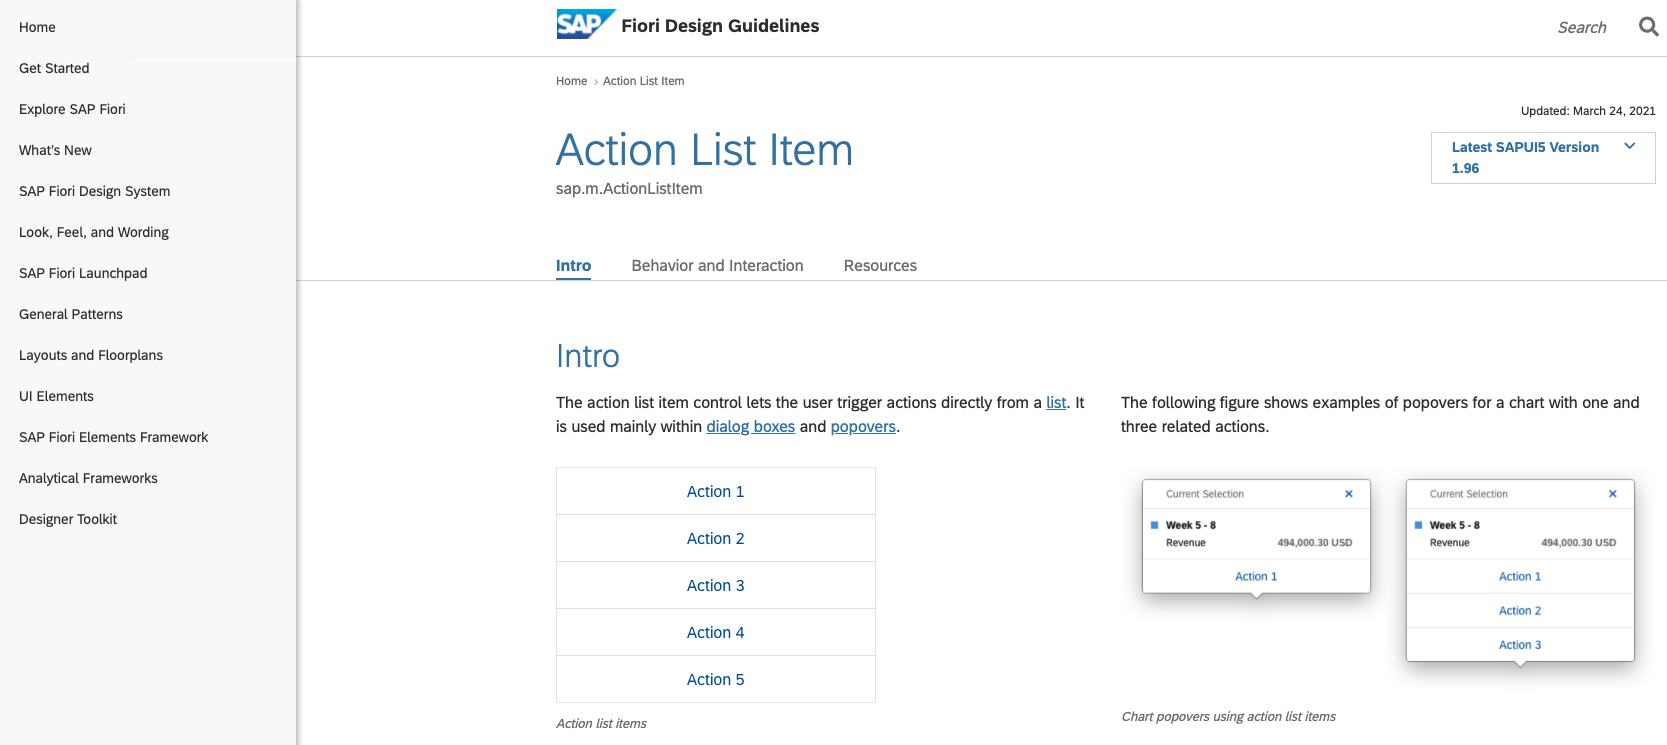
\includegraphics[width=\linewidth]{images/fiori_action-list_formal.png}}
\caption{SAP Fiori Action List formal guideline \cite{sap_fiori_action_nodate}}
\label{fiori_action_list}
\end{figure}
\paragraph*{Usage guidelines} Here the questions should be clarified how to use the components. Furthermore, the parameters and their use are explained. The user should know from this documentation how to configure and use the component. \cite{vesselov_building_2019}
\begin{figure}[htbp]
\centerline{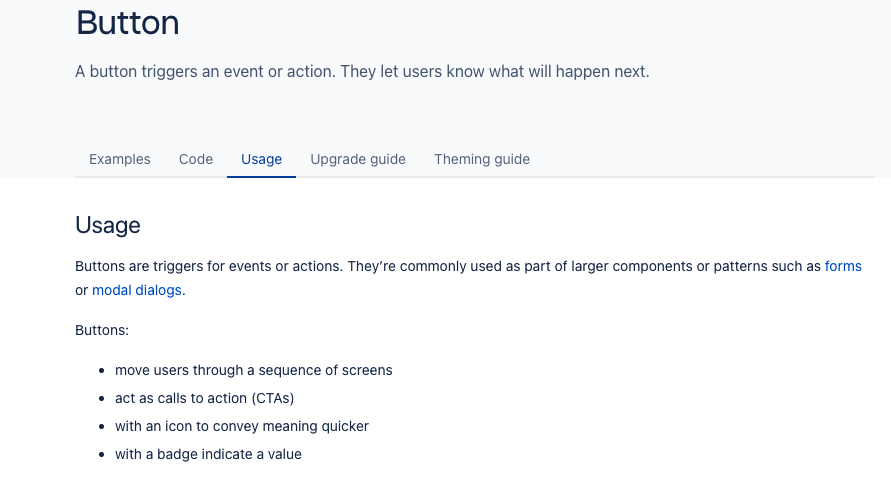
\includegraphics[width=\linewidth]{images/atlassian_button_usage.png}}
\caption{Atlassian Design System Button usage guideline \cite{atlassian_button_nodate}}
\label{fiori_action_list}
\end{figure}
\paragraph*{Technical guidelines} \label{tech_guideline}
This part of the guide is mainly intended for developers who are to implement the documented component in the software. Any ambiguities about the implementation should be clarified here. Also how the presented parameters can be used to configure the component. An often found feature here is copying code snippets. This allows developers to immediately copy-paste the component code they have just read into their code.  \cite{macdonald_practical_2019} \cite{vesselov_building_2019}
\begin{figure}[htbp]
\centerline{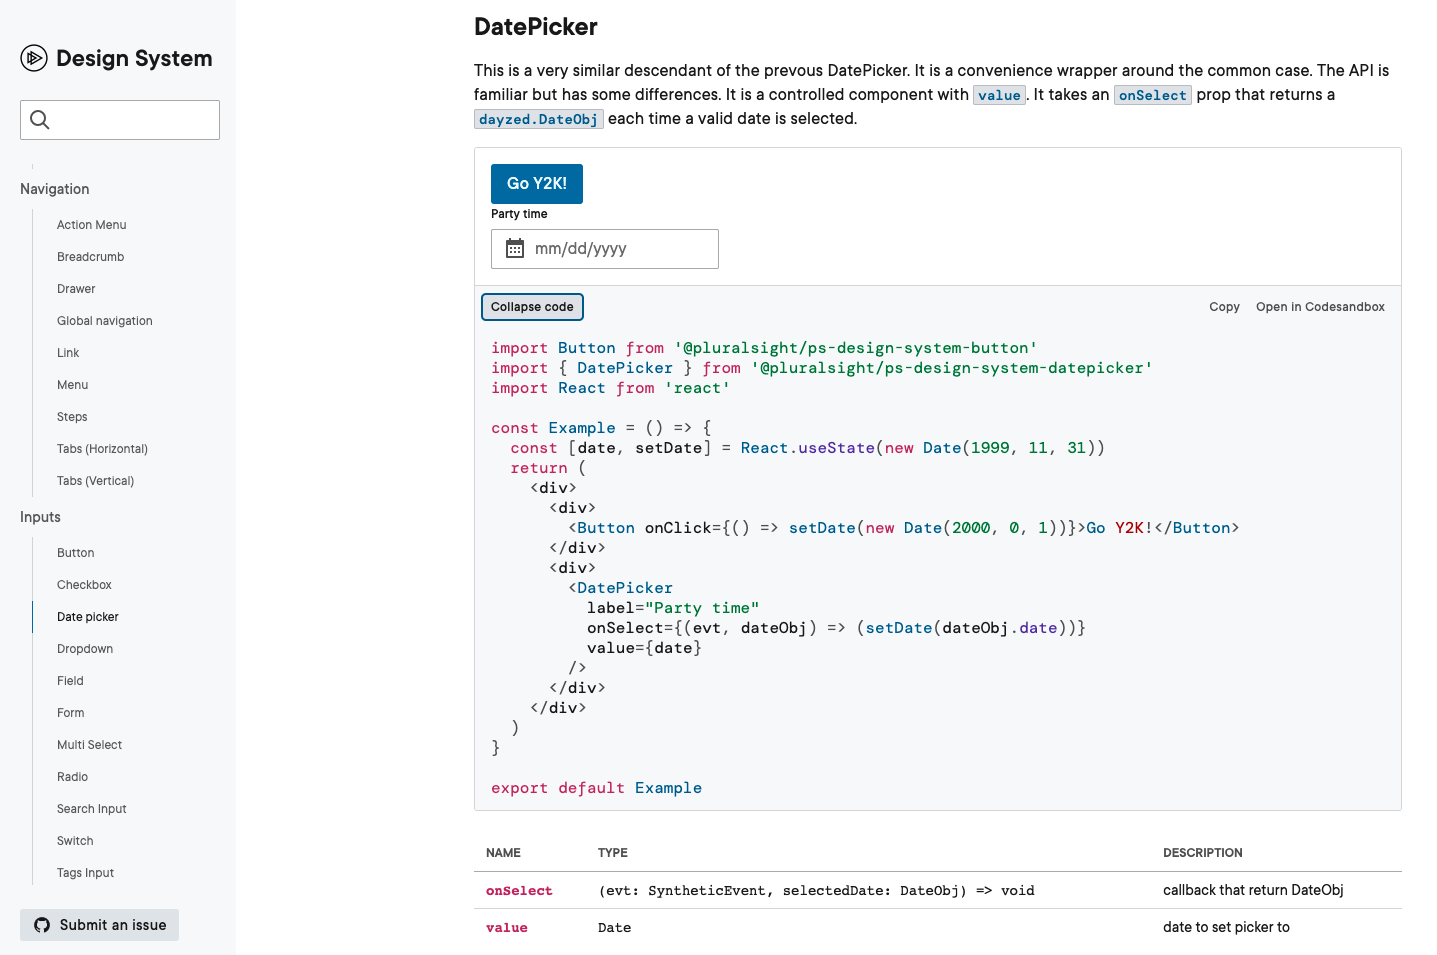
\includegraphics[width=\linewidth]{images/pluralsight_date-picker_technical.png}}
\caption{Pluralsight Design System Date picker technical guidelines \cite{pluralsight_datepicker_nodate}}
\label{fiori_action_list}
\end{figure}
\paragraph*{Related components} Linking components and regions help the user explore the design system. Also, this can help the creative process for designers and developers.  \cite{vesselov_building_2019}
\begin{figure}[htbp]
\centerline{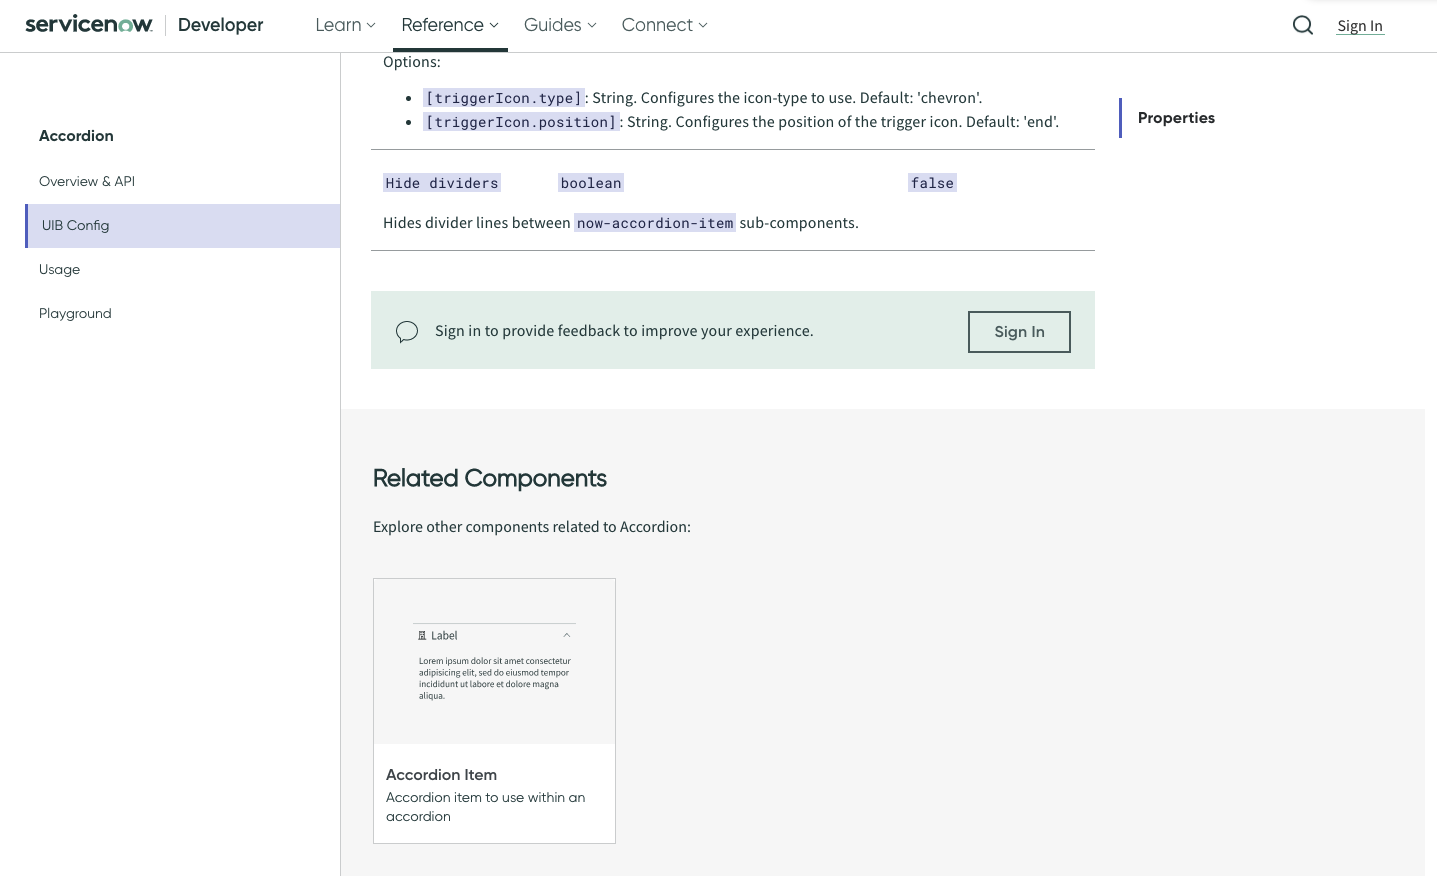
\includegraphics[width=\linewidth]{images/servicenow_accordion_related.png}}
\caption{Servicenow Accordion related components \cite{servicenow_now_nodate}}
\label{fiori_action_list}
\end{figure}

\subsubsection{Design Principles}
Design principles should be a central consideration when building a design system. In doing so, design principles should reflect the norms and values of the product organization.  In doing so, the points established do not follow any rules, except that they are established collectively by the team.  \\
Thus, these design principles serve as a basis for discussion and decision-making for designs. By simply self-explanatory principles it is possible for the designers and developers to quickly create new designs without a large coordination effort. Often questions are taken as principles. This gives developers and designer an impulses to ask themselves if they are aligned with the design principles during the creation process. \cite{brignell_design_2022} \\
As an example there are design principles for the Web by \citet{berners-lee_principles_2013}: 
\begin{itemize}
\item \textbf{Simplicity} - Simple solutions are better solutions
\item \textbf{Modular Design} - Change things and it will only affect one part
\item \textbf{Being part of a Modular Design} - Realize you own the Design System
\item \textbf{Tolerance} - "Be liberal in what you require but conservative in what you do"
\item \textbf{Decentralization} - Don't produce bottlenecks, allow scaling in any direction
\item \textbf{Test of Independent Invention} - "Designing a system not to be modular in itself, but to be a part of an as-yet unspecified larger system."
\item \textbf{Principle of Least Power} - Use matching tools for the matching tasks
\end{itemize}
Design principles can be quite different. In this case, they are relatively technical, as the team wants to focus on these issues. Other organizations, such as Adobe (\url{https://spectrum.adobe.com/page/principles/}), have people at the forefront.  \\
The design principles play a central role in a design system. The importance these anchor points is often underestimated. The product team should not only build software based on these principles, but also gain an understanding of the big picture of the product organization. Thus, design principles should be aligned with the design strategy of the company.  In this way, not only is the existing product organization aligned with the design principles, but new employees can also use them to more quickly integrate themselves into the product organization.  Design principles are effective when they serve as a guide for the creative process.\cite{vesselov_building_2019} \\
In order to apply design principles, they must first be created. While it would be possible to create them yourself, it is not recommended because these principles are intended to reflect the creative thinking of a large group of the product organization. Here, \citet{vesselov_building_2019} lay out a 5-step plan to iteratively create and continuously improve them. In the following figure \ref{design_principles_steps}, these 5 steps can be seen:
\newpage


\begin{figure}[htbp]
\centerline{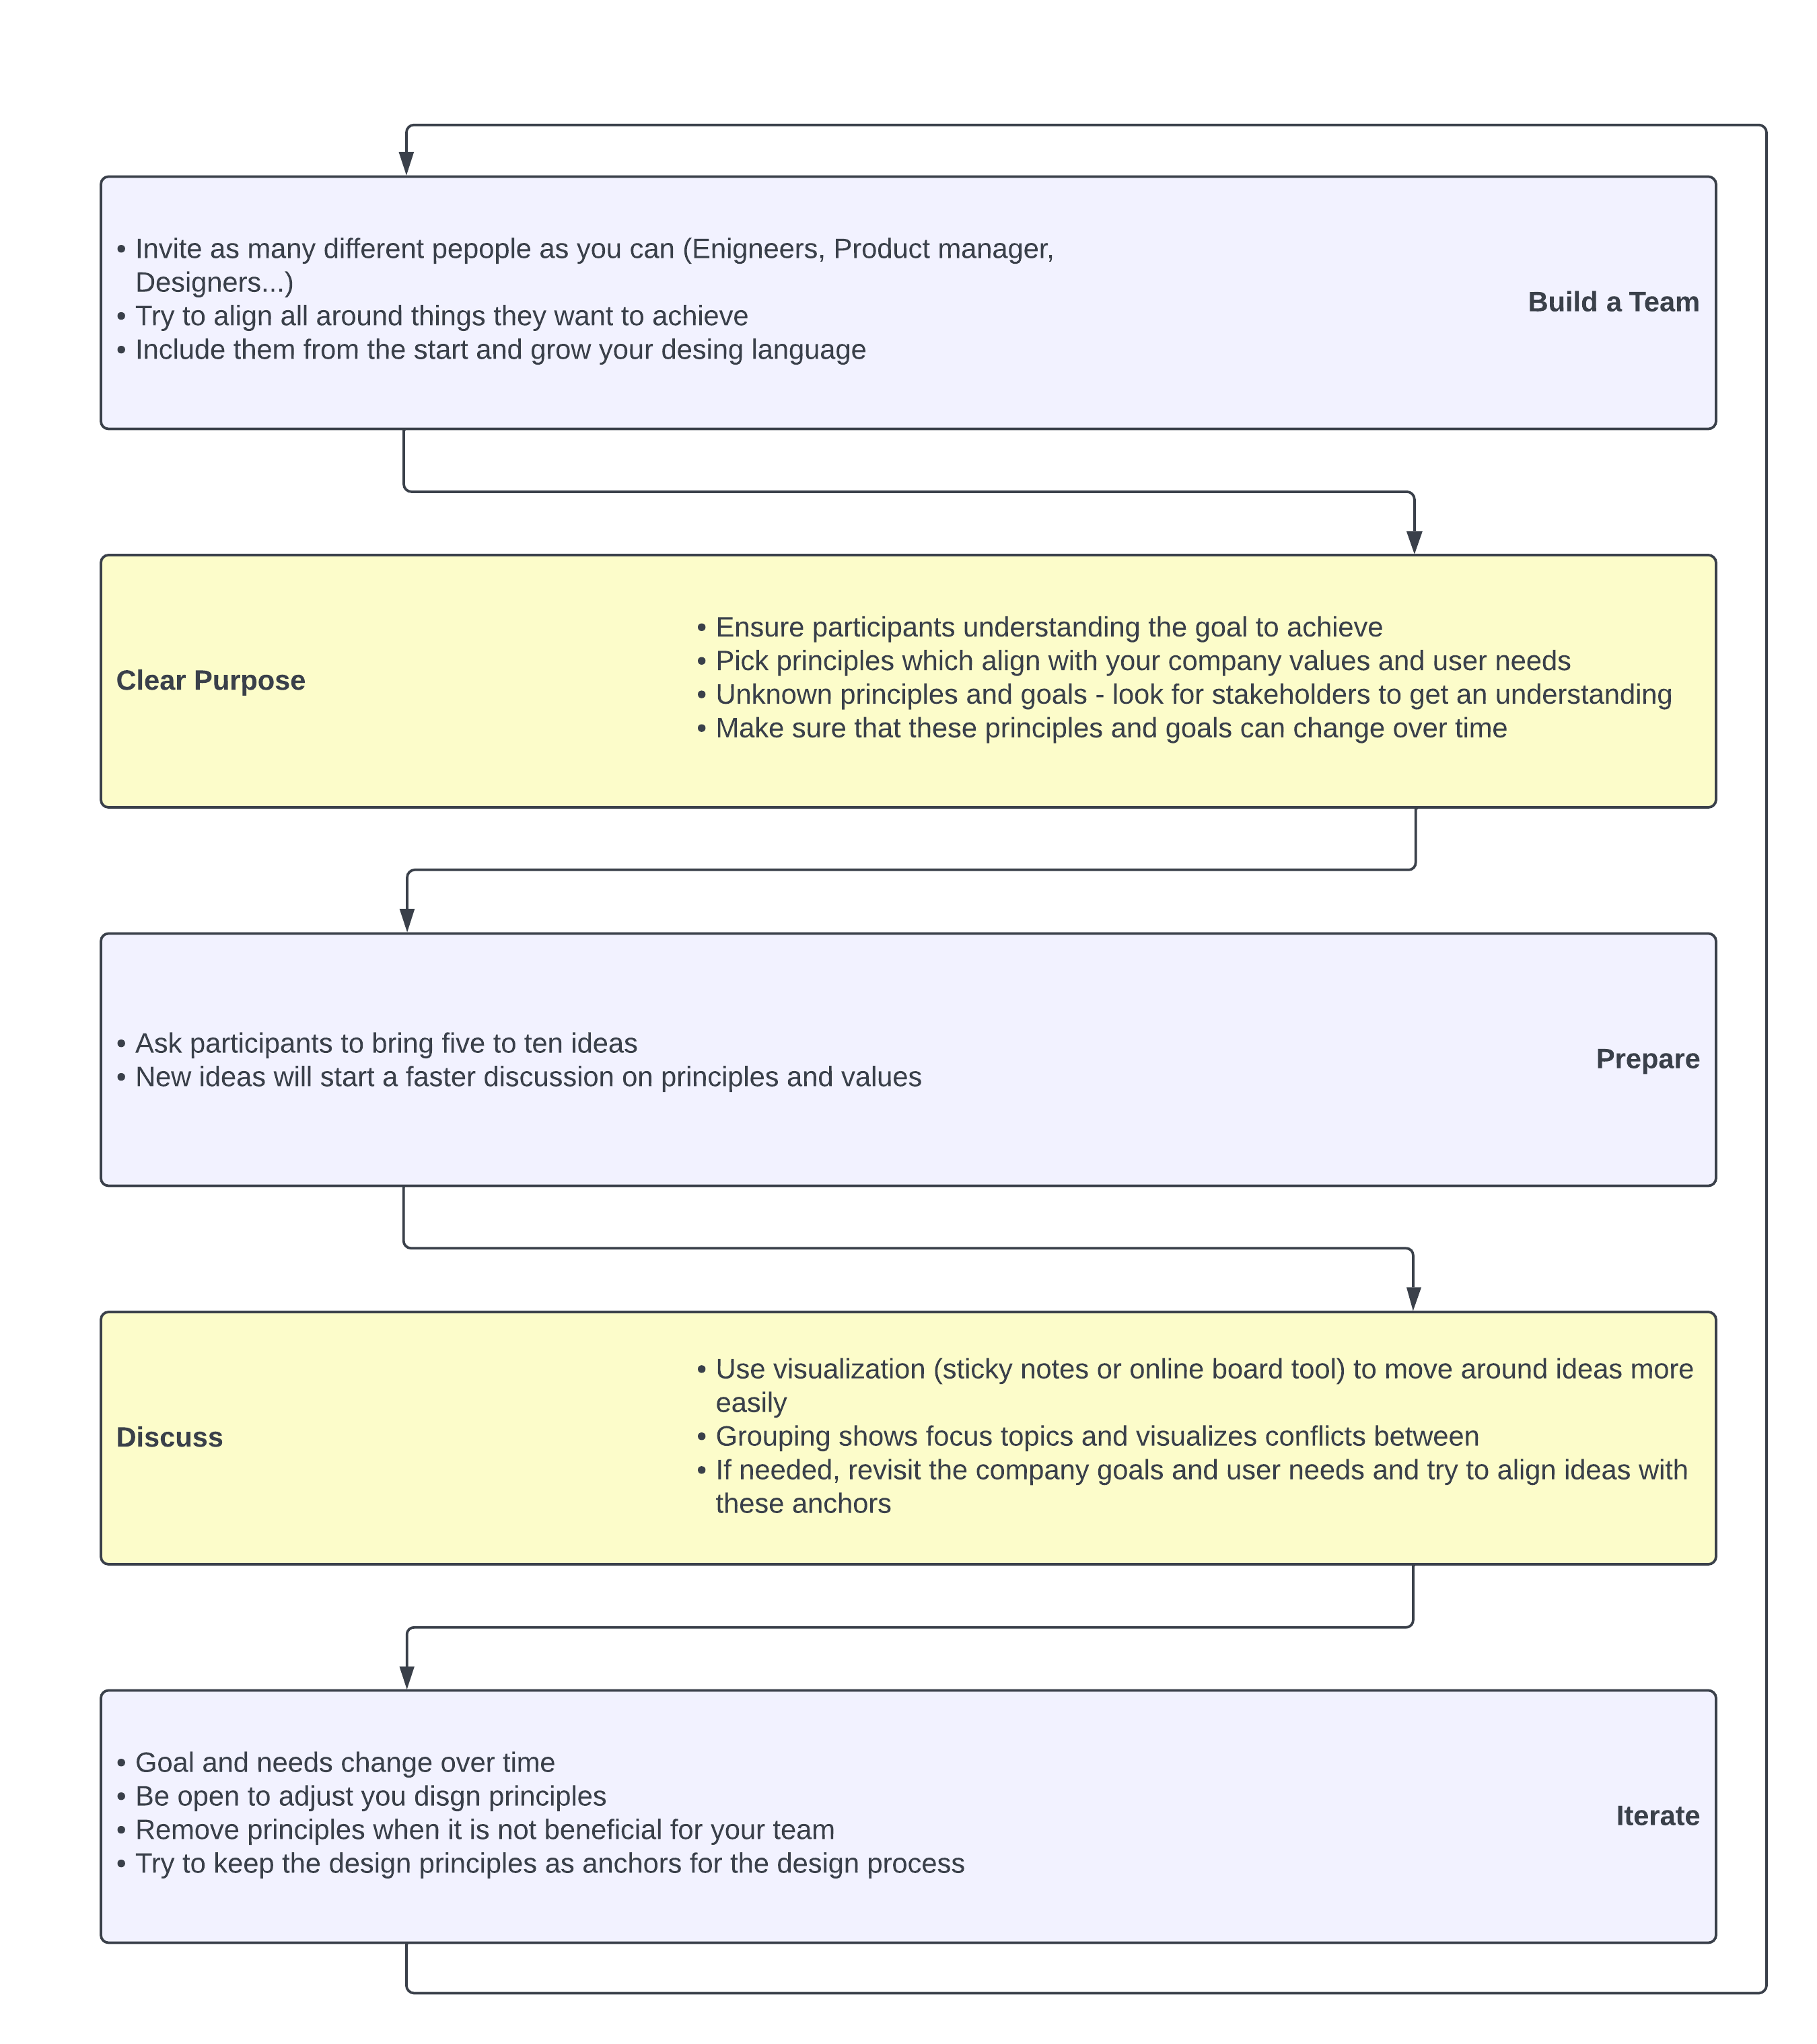
\includegraphics[width=\linewidth]{images/design_principles_steps.png}}
\caption{5 steps to introduce design principles inspired by  \citet{vesselov_building_2019}}
\label{design_principles_steps}
\end{figure}
Once design principles are in place and an iterative process to keep them up to date is installed, there is a need to share these principles with the rest of the product organization. This is where many design systems offer what are called design blogs or design news. They not only help the organization keep track of the design principles in their daily work. They also provide a platform to share updates with users.  Moreover, there is an exchange on related topics on these platforms. This in turn helps to improve and keep the design system and design principles up to date.  \cite{google_material_2022}\\

Having set the foundation with the guidelines and design principles, the next chapter will deal with another important building block, the component library.
\subsubsection{Component Library}
The technical counterpart to the description guidelines and design principles is the component library. Both cannot exist in a design system without each other.  By definition, a component is "a constituent part" \cite{component_definition} of in this case a user interface.  Combined with library, which means a "collection of something"\cite{library_definition}, it results in a collection of important constituent parts for user interfaces.  \\
The definitions existing from the literature are as follows:
\begin{tcolorbox}[title=Definition of component library by \citet*{vesselov_building_2019}]
A set of styles and components that can be used and shared among a team. A component library consists of common core elements that are used throughout an application. [...] Component libraries may or may not include living code. [...] Unlike UI frameworks such as Bootstrap, component libraries are tailored to specific purposes, like an internal brand.
\end{tcolorbox}
In addition to components, there are also styling rules that also include layout specifications in component libraries. 
\begin{tcolorbox}[title=Definition of component library by \citet*{macdonald_practical_2019}]
Component libraries, UI libraries, or code libraries provide frontend code for UI components (a.k.a. widgets, modules, chunks, blocks). Internally, you might use a component library as a shared collection of UI snippets implementing patterns that anyone in the organization can contribute to building.
\end{tcolorbox}
An important point that emerges from these definitions is that component libraries have a clear focus on internal use. This is also the main difference to UI frameworks. \\
After reviewing various design systems, their component libraries can be split into the following 4 points:
\begin{itemize}
	\item \textbf{Layout} - Spacing and presentation of content placement on a site
	\item \textbf{Styles} - Color definitions, Typography, Icons
	\item \textbf{Components} - Reusable parts fulfilling one purpose
	\item \textbf{Regions} - Combination of multiple components 
\end{itemize}




% Six interlocking areas make up a design system: layout, styles, components, regions, content, and usability. A robust design system should contain guiding design principles, guidelines for use and implementation, as well as a component library that includes front-end code. \cite[p.23]{vesselov_building_2019}

% Vesselov ab Seite 71
% https://design-system.service.gov.uk/
% Wie GOV AUS 

% https://www.bbc.co.uk/gel
% Kein Komponenten sondern Fokus auf Patterns, Foundation als Principles
\paragraph{Layout}
The foundation of any design system is the ability to place, move, or arrange elements on web pages. To achieve a consistent appearance, it is important to align spacing and positioning. 
For this purpose, so-called design tokens in the form of CSS variables are often used. Similar to Tailwind (\url{https://tailwindcss.com/}), these variables are then translated into CSS classes so that the developer does not have to use the variables natively. And thus does not need to know CSS.  \\
Salesforce Lightning Design System, for example, lists all layout tools under "Utilities." It sets sizes for text, simple boxes, and spacing between components. In fact, a sophisticated grid layout system can be seen as well. \\

IMAGE

As can be seen, CSS classes are used to achieve the desired layout. Both dynamic and static layouting are supported. So the user has all the possibilities to use the layout of the design system. \\
Besides the usual regulations for spacing and positioning, other points like visibility, scrollability or printability can also be described in the layout. Basically, all requirements for visible elements in the target system can be specified by the default layouting in the design system.

\paragraph{Styles}
Styles are about colors, typography and icons. Here it is important to establish a connection to the chosen design principles. This helps to better convey the overall design language in the next steps. 
It is important to mention that when using the style theme in multiple products, there should be a possibility to configure it. This way, each product can still have a unique look and feel. \cite{vesselov_building_2019}
\subparagraph{Color}
The introduction of a color system is a good first step on the way to a design system. Colors are important for the aesthetics of a product and can be easily iterated and changed without changing functionality or layout. It is always important to keep accessibility in mind when choosing colors. For certain text sizes, it is important to maintain a certain contrast. The WCAG (\url{https://www.w3.org/WAI/standards-guidelines/wcag/}) describes this contrast with two levels AA and AAA. This contrast is especially important if the product has several long paragraphs.  \\
Usually, not a single color is created, but an entire palette. The colors are often divided into primary, secondary, text color, background color, accent colors, shadows and so on. Also here CSS variables with the appropriate names are created to use them. The challenge is to offer a well-defined color palette, but at the same time not to overload the user, because with too many colors the overview gets lost quickly. \cite{vesselov_building_2019}


IMAGE 


\subparagraph{Typography}
When it comes to a typography system, it can be divided into two categories of typography. First, there is typography that is used for two or perhaps three words at a time, such as headings or button elements. Second, there is defined typography for longer texts such as paragraphs. \\
In both cases, it must follow the defined layout system. Important things like baseline height, padding, and margins are important here. A helpful piece of advice is to represent all types of text possibilities in your typography system.  \cite{vesselov_building_2019}


IMAGE

\subparagraph{Iconography}
There is no need to create iconography with each new design system. In the wild, there are many good options that can be used right away. But creating a new iconography provides many opportunities to visualize your own design language in the iconography.
\\
As with other parts of a design system, documentation is key. How to create new icons, what proportions and shapes are important. If done right, it's an easy step to introduce new icons into the iconography. 
\\
To make them accessible to the team, there should be a description of how to add them to the software. There should be the same representation of the source code as in the technical guidelines in \ref{tech_guideline}. \cite{vesselov_building_2019}


IMAGE
\paragraph{Components}
With all the tools and fundamentals in hand, the main part of a component library, the components can be assembled. Components should be highly reusable and as flexible as possible. They represent building blocks of applications.  \\
From combinations of layout and style specifications components emerge for different use cases. By using these defined components within applications, the developer ensures that guidelines are followed. For certain combinations of components in an application, there is another term called regions, which is explained in more detail in the next chapter \ref{regions}. \\


EXAMPLE OF COMPONENT


DOCUMENTATION EXAMPLE


In order to achieve flexibility and reusability, it is important to have always the interfaces of the component in the mind. Well defined interfaces are the key to successful components. To achieve this, always involve the engineers building the actual product to get their feedback on the interfaces. As with other parts of a design system, documentation is key. A well-structured and systematic approach to how a component works helps developers use the components.  \cite{vesselov_building_2019}



INTERFACE EXAMPLE
\paragraph{Regions} \label{regions}
Often, a combination of certain components is used over and over again in different places and even in different applications. To cover this use case, a design system has a concept called regions. Regions specify a combination of several components and document the use and composition of these components. They can be seen as an extended documentation to reproduce a certain behavior in an application. 
\\
Regions refer not only to the interaction of components, but also to the switching of visualization due to changes in a user's permissions, for example. All these types of UI-related documentation needed to define a particular user experience can be documented here.   \cite{vesselov_building_2019}
\\
Most often, regions appear in the general navigation of applications. They evolve naturally from the finished products and grow iteratively with more and more feedback from the product development team.
\\
A good example is the navigation bar. Components such as buttons and dropdown components can be used in combination with the skeleton of a navigation bar to create the region called Navigation Bar. 

%% \subsection{User Experience}
\\
\\
In summary, design systems are a complex but powerful construct for creating modern software. This elaboration of the design system lays the foundation for building a design system that serves as the basis for a whole range of applications. How and in which steps this is done is described in the next chapter. 
\newpage
\section{The \ac*{SDS}}
This chapter presents the implementation of the newly created design system as a standard for the web user interfaces for SaaS products. \\
First, a look at the architecture and modelling is taken. Looking at existing design systems and trying to understand  how they work and extract requirements in order to develop a common system that fits most products in the SaaS world. \\
After that this chapter presents an actual implementation of a component, including the technology stack used and how the components are built. \\
Finally, the build chain is explained. Including all information on how components and atoms are consumed and bundled. Also giving an outlook what is needed to get the SDS running inside a existing or new project.
\subsection{Architecture}
Modelling the architecture of a system that supports customization of SaaS product user interfaces is not a trivial task. Often, user interfaces for products are developed only to support their purpose. Finding common ground for multiple products can be difficult.  \\
Design systems define a common place where the company's products can align. Why is it not possible to develop a central system to create a common idea for user-friendly SaaS products? Not only do well-designed components help align, but a design system foundation with guidelines and principles helps developers and designers create a good product. \\
To this end, 10 different design systems of well-known SaaS products, as well as design systems with a shared purpose, were considered. 
\begin{table}[!ht]
\begin{tabular}{|p{0.2\linewidth} | p{0.7\linewidth}|}
\hline
 \textbf{Name} & \textbf{Description} \\ \hline
Service Now  & Platform design system.  Guidance to create components and upload them to the platform. \\ \hline
Adobe Spectrum  & User centralised design system. Many well designed components with matching guide to deliver a great experience. Built in web components and react components. \\ \hline
Zendesk Garden & Basic design system with guidelines, components and patterns. Tailwindcss integration. Built in react components. \\ \hline
Atlassian Design System & Design System connected with company values. A lot of guides on how to use designs, components and to write content. Includes also employee motivation. Built in react components. \\ \hline
Base Web  & Open source design system. Used by Uber. Providing a blog and guides on how to use the base design system. Design System intended to be used as baseline and should be overwritten when used. No principles or values included. \\ \hline
SAP Fiori  & Standard design system. Focus on accessibility and multiple device support. Including many themes for different applications. Delivers a toolkit to better use the design system as a designer.  \\ \hline
GOV UK Design System  & Not really a design system. Missing guidelines and principles. Externals can propose changes. Providing CSS classes for HTML elements.  \\ \hline
Lightning Design System & Design System to support developers and designer at their work. 4 principles with a clear message to align every user. Guidelines and best practices on many topics.  Components are built with pure CSS classes. \\ \hline
Google Matrial Design & Open source design system. Providing the user with design principles which helps to understand the usage of the design system. Material Design provides only components and no patterns. Blogs and further resources are helping additionally to the guidelines. Components are built with pure CSS classes. \\ \hline
Pluralslight Design System & Design System without principles and guidelines. For the moment only components are present. Providing a workflow for developers and designers to contribute to the design system.  Only few patterns. Built with react components.  \\ \hline
\end{tabular}
\caption{\label{tab:design_systems_in_the_wild} Overview of 10 existing design systems}
\end{table}
As can be seen in table \ref{tab:design_systems_in_the_wild} fot these 10 examples of design system, the interpretation of one can vary. \\
A good reference for a design system with a suitable use case is the Base Web Design System. Its purpose of providing a base of styles and functional components helps developers customise for their products. Also, the fact that this design system is open source underlines that this design system has been developed by the community and is not controlled by a corporate design team. Built-in accessibility is also a requirement that must be present in a common design system. The instructions on how to extend and use the design system are also a perfect reference. \\
But there are also disadvantages. The Base Web Design System lacks guidelines and principles that are crucial for a design system. A look at Google's Material Design shows that even an open-source and versatile design system can have design principles. Design principles help developers get an idea of how to develop and design with the system. Therefore, design principles are indispensable in a design system and should not be missing. \\ \newpage
Another reason, is the use of React for creating the components in the Base Web Design System. As a design system that should be used by everyone as a standard for the implementation of SaaS products, it is therefore unsuitable. As developers are expected to use React as a frontend library. Looking at other examples such as the GOV UK Design System or Salesforce's Lightning Design System shows that it is possible to create components using web standards that can be used by anyone without having to use a library. \\
With these requirements, an architecture can be drawn as can be seen in figure \ref{architecture_sds}. \\
\begin{figure}[htbp]
\centerline{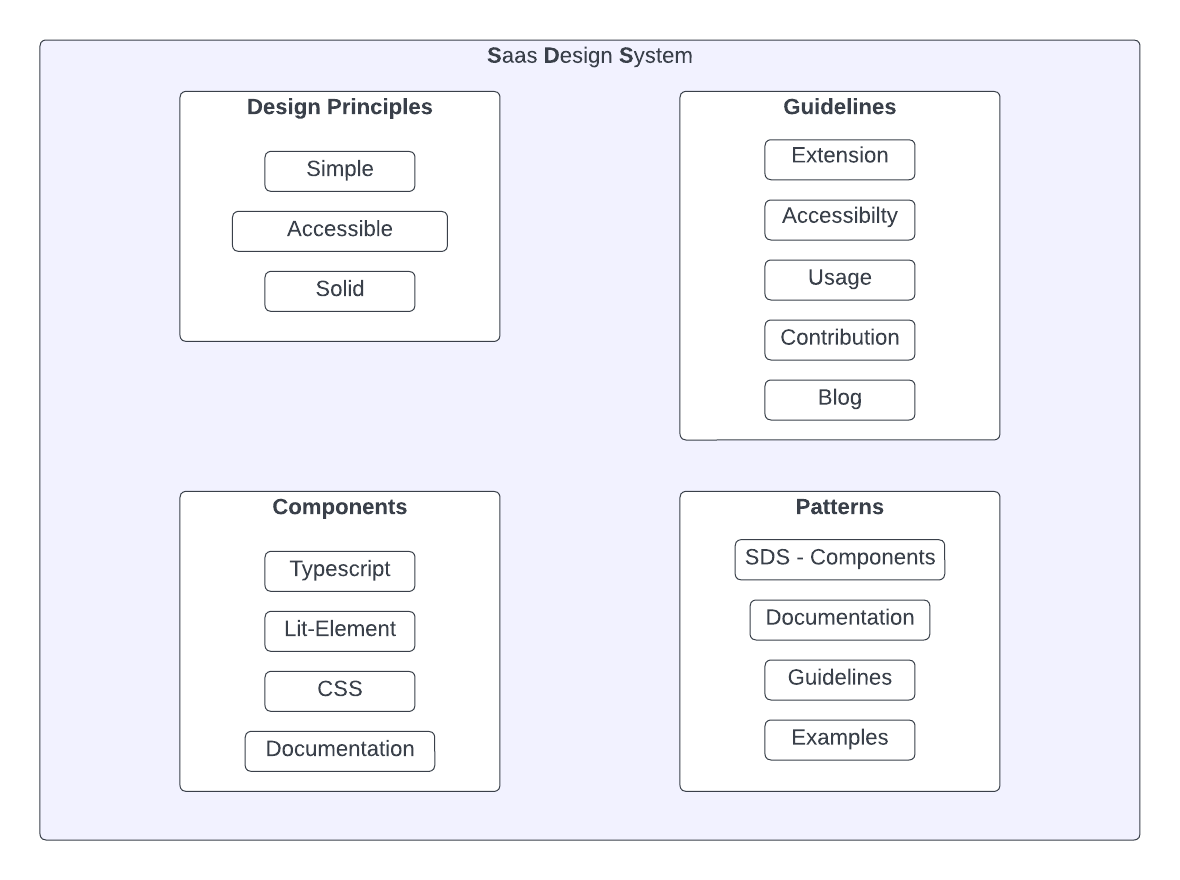
\includegraphics[width=\linewidth]{images/architecture_sds.png}}
\caption{Architecture of SaaS Design System}
\label{architecture_sds}
\end{figure}
According to the description of a design system presented in chapter 2, the SaaS design system can be roughly divided into four parts.
\subsubsection*{Design Principles}
In terms of design principles, the SDS strives to keep them lean and easy to understand, as the design system is intended to serve as a basis for other design systems. The \textbf{Simple} principle states that component design should not have unnecessary styles or features that make it difficult to extend. \\
Many products strive to implement accessibility in their products. With the \textbf{Accessible} principle, SDS emphasises the importance of accessible user interfaces. This is not only important in terms of inclusion, but also helps accessibility in the overall user experience for all users. \\
The third and final principle is \textbf{Solid}. As stated earlier, the SDS should be a foundation for other design systems to build upon. Therefore, the importance of a stable and consistent API is very important. For this reason, the design system has deliberately chosen \textbf{Solid} as the third and final principle. \\
\subsubsection*{Guidelines}
The SDS guidelines are based on the design principles just presented. In addition to the core guidelines on extension, accessibility and basic use, there are also guidelines that focus on contributions and collaboration. As this is an open source system, as many people as possible should be able to work on it. \\
The extension guidelines address how to integrate SDS as the basis for a company's own design system. It shows developers and designers how to create their own from the components provided. \\
Since accessibility is also a design principle, there must be a guideline that defines what the SDS means by accessibility. It should give the user a definition and sources for accessibility. But also self-designed components should have a guideline that helps users to implement accessibility. After this guideline, the user should have no more questions about accessibility. \\
As a third guideline, the SDS will support the user in using the system. This guide could also be seen as an entry guide and will cover the basics. Importing the design system, proper bootstrapping and guidance on configuring the system. This may seem self-explanatory, but lacking these often prevents users from using the system effectively. The user guide should be as simple as possible and cover every small step needed to get started with the SDS. \\
One goal of this design system is to be developed by the community for the community. However, this can quickly get out of hand if everyone contributes without any guidance. Therefore, it is important to introduce some from the beginning. This guide provides guidance on how to contribute to the component library, but also on how to enforce changes to the guidelines and principles. As this design system is not set in stone, there should be opportunities to change and adapt everything. What this will look like in the end will evolve over time. Some ideas could be a voting process or an RFC (source) process, as is common in the software industry. \\
To achieve high interactivity in such a design system, some design systems introduce blogs and forums for knowledge exchange. In this way, users can connect, discuss and contribute to ideas to further improve the design system. The most important point is the moderation of such an interaction platform. A well-moderated blog and forum will further enhance the community around the SDS. \\
Overall, it can be said that the guidelines for the SDS are aimed at building a community around the design system to contribute and enable users to create a community design system. 
\subsubsection*{Components}
Without well-assembled components, design systems cannot exist. Therefore, choosing the right technology package for building components is very important. 
In the case of SDS, one of the most important requirements is that the system is usable independently of the front-end framework used. To achieve this, SDS uses the web components that are supported in almost all modern browsers. As it is possible to create web components without importing libraries or frameworks, it is a perfect complement for SDS. (Source)\citep{component_definition} \\
Creating web components natively can be complicated. For this reason, the Lit framework was designed to make it easier for developers to create web components. With a focus on ease of understanding, intelligent DOM updates and small package size (5 KB), Lit is a perfect complement for creating components for design systems based on standard web components. \citep{component_definition} \\
To further assist developers, SDS uses Typescript, a superset of Javascript. It extends Javascript with types and interfaces. Typescript must be compiled into Javascript for the browser to understand it, but this allows the developer to find errors much faster because it fails at compile time rather than at runtime. \citep{component_definition} \\
To use and provide design tokens for colours or spacing, the SDS uses custom CSS variables. They are imported into the root element during bootstrapping of the design system. The definition of the design tokens can be found in the documentation. \citep{component_definition} \\
Last but not least, the design system components created must be documented and accessible to users. To start SDS, Storybook is used, which has a lot of built-in functions that support documenting the components. With MDX, the combination of Markdown templating (MD) and code injection via JSX, it is possible to write fluid documentation without having to jump back and forth between files. \citep{component_definition} \\
With this technology stack, SDS provides users with highly reusable web components that are not only easy for users to access, but also easy for contributors to develop. 
\subsubsection*{Patterns}
An essential part of the SDS are the patterns. They describe how user interfaces should be designed to align with the core capability of this design system. The patterns help developers automatically apply best practices and web standards without having to read an entire text. \\
Patterns are created using components and standard HTML elements provided by the design system. These are easily accessible to the developer by copy and paste. With additional documentation on when to use them and when not to use them. \\
The patterns are supported by additional guidelines on how they can be adapted and redesigned. This enables developers to meet the requirements needed for their own design system.\\
Accordingly, live examples show the developer how the patterns will work in the final product. With several different examples for each pattern, the possibilities for customising each pattern are presented. SDS users also have the opportunity to share their creations and application of patterns below the documentation. 

\subsection{Design System Components}\label{sds_button}
An important part of the implementation of a design system are the components. As described in chapter \ref{sds-component}, the components are created using the Lit framework. To see a complete example of a component constructed with design tokens and documented with the storybook, the example of the button component of the \ac{SDS} is presented in this chapter. \\
The components use TypeScript to take advantage of custom decorators. The decorators provided by Lit further simplify the boilerplate code for creating a web component. \\
\lstinputlisting[linerange={1-4},firstnumber=1,caption={Initialization of \ac{SDS} button component},label=ButtonInit]{../Code/src/components/button.component.ts}
In listing \ref{ButtonInit}, the component is initialised with the \texttt{@customElement} decorator by passing the tag name as a string and appending it to an \ac{ES6} class. For it to work properly, the class must extend the Lit Element class. When everything has been implemented as described, the web component is registered and can be used with the defined tag, in this case \texttt{<saas-button>}. \\
In order to see something when the web component just created is used, it must implement the render method. This method expects a \texttt{TemplateResult}. 
\lstinputlisting[linerange={19-26},firstnumber=19,caption={Rendering of \ac{SDS} button component},label=ButtonRender]{../Code/src/components/button.component.ts}
Lit element provides the import of a \texttt{html} string literal that can be used to construct the \texttt{TemplateResult} expected by the render function. With this functionality, Lit provides an efficient way to respond to variable changes and intelligently update the \ac{DOM}. \\
Properties also make use of custom decorators and declare properties on web components by writing \texttt{@property} in front of a class attribute (line 19-20, Listing \ref{ButtonRender}). Thus, Lit Element implements change detection and adds automatic type conversion. For a detailed description of the capabilities of this decorator, see the documentation. Whenever the property value of the created button web component changes, the constructed template string reacts to these changes and updates the displayed template accordingly. \\
Last but not least, the web component must use the defined design tokens. Since these tokens are defined by \ac{CSS} variables, they can simply be consumed as follows: 
\lstinputlisting[linerange={5-20},firstnumber=5,caption={Styles of \ac{SDS} button component},label=ButtonStyles]{../Code/src/components/button.component.ts}
The Lit Element framework implements a static property of the \texttt{styles} to its classes. To make it work properly, a string literal \texttt{css} is used to convert a string into the required \texttt{CSSResult} type. In this way it would be possible to consume design tokens via input properties, but to simply manipulate design tokens in one place, the components of \ac{SDS} will use \ac{CSS} variables. In this way, it is possible to customise certain tokens throughout the design system by adapting these tokens. Each component in the \ac{SDS} will use the defined tokens. Line 7-9 in listing \ref{ButtonStyles} shows an example of the use of design tokens for the button component in the \ac{SDS}. \\
Finally, the button component is displayed in Storybook, the documentation tool for \ac{SDS}. Limited to the time frame of this elaboration, the documentation is kept short. Figure \ref{storybook_button} is an example of what the documentation of \ac{SDS} components may look like. A full version of documentation as in other mature design systems will have to be added in a subsequent development of \ac{SDS}. \\
\begin{figure}[htbp]
    \centerline{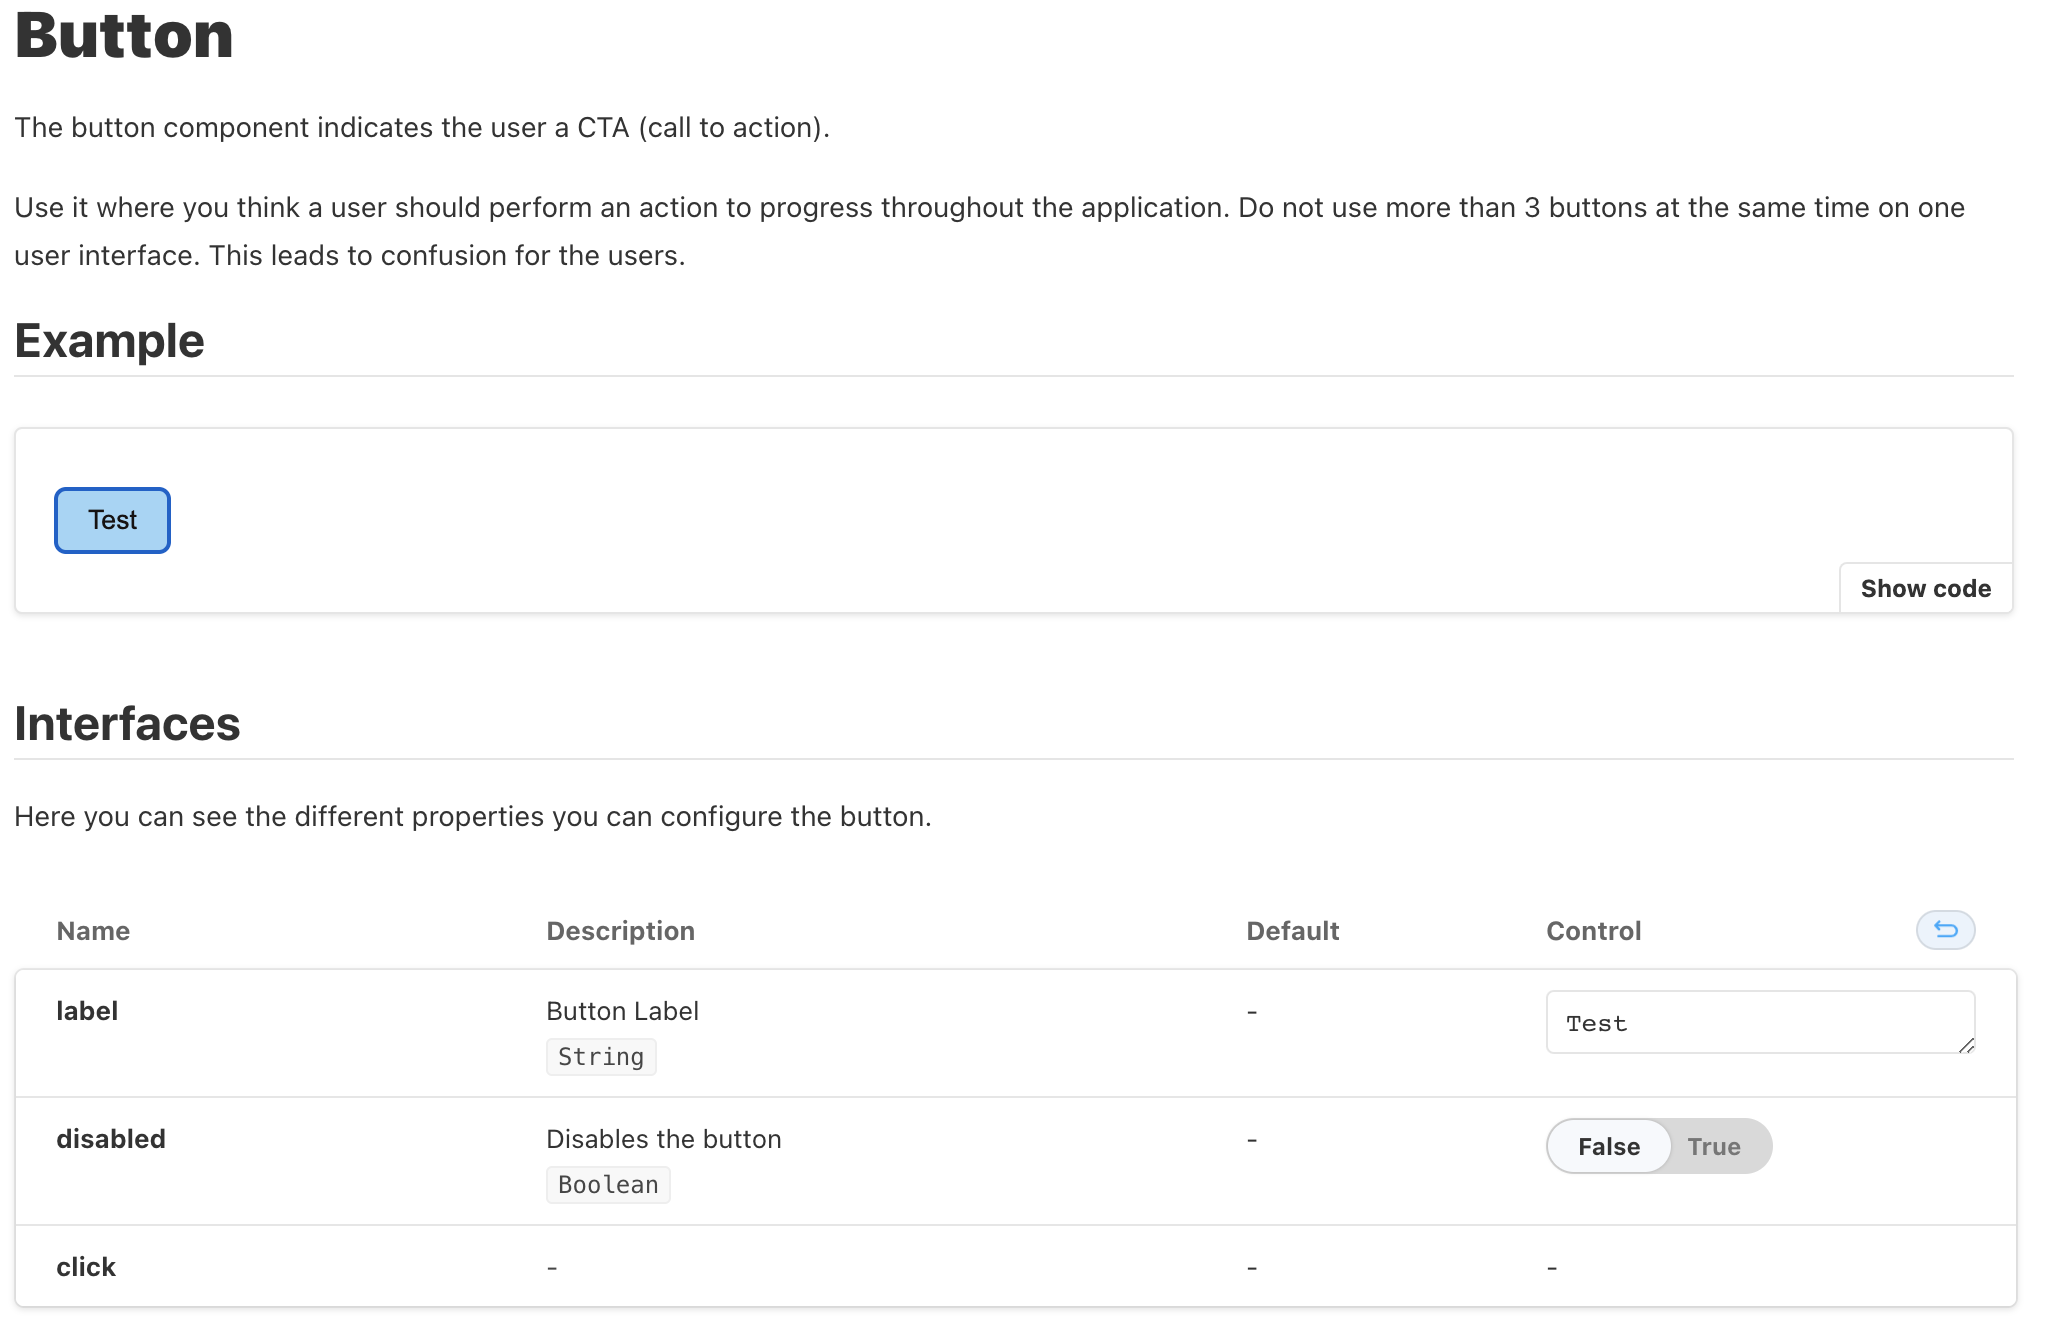
\includegraphics[width=\linewidth]{images/storybook_button.png}}
    \caption{Example documentation of the \ac{SDS} button component}
    \label{storybook_button}
\end{figure}
At the moment, the documentation consists of a short description that briefly explains to the developer how and where he can use the button in his applications. In addition, a live example of the component is presented, which is automatically linked to the properties shown below. When the properties are changed, the example above is updated. This means that the developer or designer who wants to use this component can find out which configuration is most suitable for his use cases. \\
Inspecting the \ac{DOM} element of the button component, the element explorer looks like Figure \ref{button_element_explorer}. When you create a new web component, the saas-button tag is a valid \ac{DOM} element. A new shadow root is opened inside the button component. This allows the web component to isolate styles and elements from the global document. The elements used to display the button component are defined in this shadow root. Also, the styles for the button are defined at the shadow \ac{DOM} level, so the rest of the \ac{DOM} tree never receives these styles. This helps to keep elements and styles separated and easy to understand. \\
\begin{figure}[htbp]
    \centerline{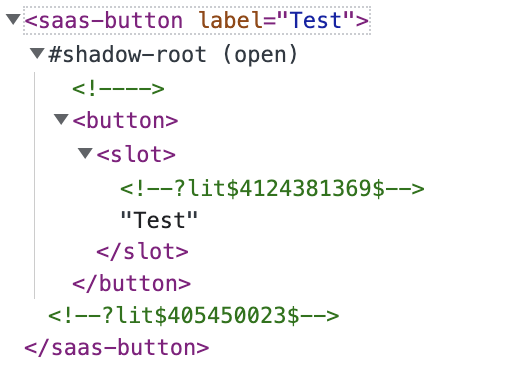
\includegraphics[height=100px]{images/button_element_explorer.png}}
    \caption{Inspection of \ac{SDS} button in elelement explorer}
    \label{button_element_explorer}
\end{figure}
It is important that \ac{CSS} variables declared in the root of the document are also available in the shadow \ac{DOM}. In contrast, style declarations, e.g. for the button element in the overall document, are not applied to \ac{DOM} elements in the shadow \ac{DOM}. \\
The \texttt{<slot>} element in the shadow \ac{DOM} is a default placeholder for anything that is inserted into the \texttt{<saas-button>} element when using the web component. The content is projected within the shadow \ac{DOM} and inserted in place of the \texttt{<slot>} element. This makes it possible to create nested elements with web components which is useful in many different use cases. \\

The example of a simple button component shows how to create and use the components of \ac{SDS}. From here it is trivial to build all the different components needed to create patterns. This is because patterns, as described, are a combination of components that can be reused in applications. The missing piece to using the \ac{SDS} in an application is integration, which is explained in the next chapter.
\subsection{Design System Integration}
The last step to complete the user story of the SDS is to integrate the system into an application. This chapter explains how to package the SDS and load it into a desired application. It is important that the integration is simple so as not to discourage developers from using the design system. \\

The build process is the first part that is important to understand the integration workflow. Webpack is the build tool used by SDS. As shown in Figure 3 in Chapter 1, the components of the design system are built using Typescript, including the Lit framework and using SCSS for styling. Since Typescript and SCSS are not supported by the browser, they must be processed beforehand. Therefore, Webpack comes into play to compile the code. \\
Webpack uses a configuration file, often called webpack.config.js, to describe the steps by which the code is compiled. This file describes rules that tell Webpack what to do with which files that come into the build pipeline. These rules for SDS look like this:\\
\lstinputlisting[linerange={23-41},firstnumber=23,caption={SDS Webpack rules},label=WebpackRules]{../Code/webpack.config.js}
The rules define regular expressions that are used to assign files with their extensions to the corresponding compilers, which are called loaders in the Webpack world. The loaders used here are build-in. But there are also custom ones that can be integrated into a build process. When using loaders, it is sufficient to include the loader string in the use property of a rule object. For example, in line 25-26, Listing \ref{WebpackRules}, the Typescript loader is matched with the regular expression Typescript to process Typescript files. The same pattern is used in line 34-35, Listing \ref{WebpackRules} to match SCSS files with the default style loader that comes with Webpack. 
\section{User Test}
\newpage
\subsection{Test applications}
The point is to have two similar applications. This way, it is possible to see if the SDS brings improvements for the end user. For this reason, both systems must be visually indistinguishable from each other. In addition, both systems contain three and one optional views that explain the test case task to the user. Therefore, the counting omits the last view.  \\

\begin{figure}[hbtp]
    \centerline{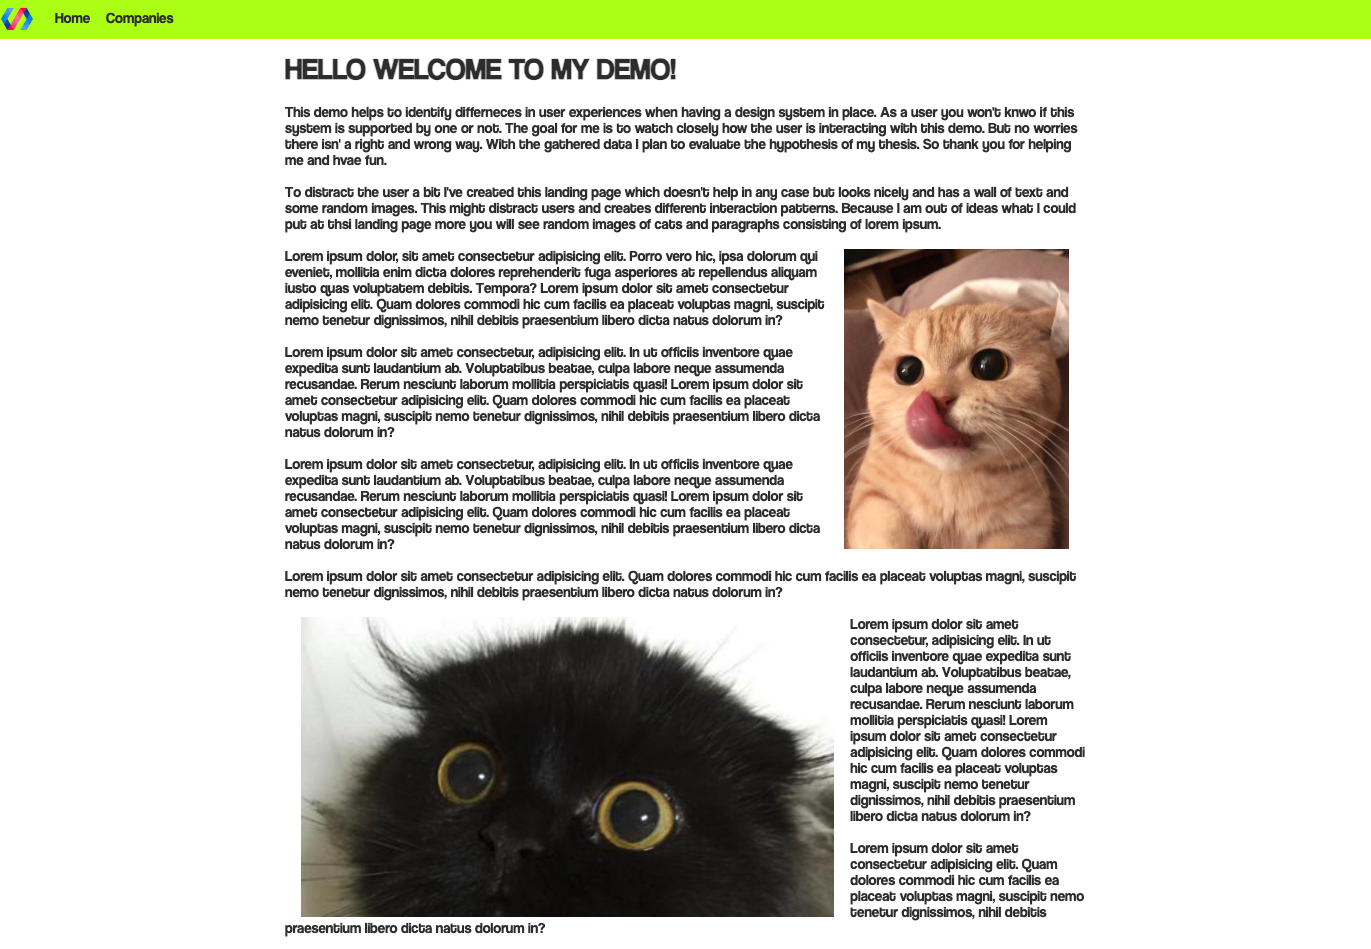
\includegraphics[width=\linewidth, draft=false]{images/demo_view_landing_page.png}}
    \caption{Landing page of test applications}
    \label{landing_page}
\end{figure}
The first view (Figure \ref{landing_page}) is the landing page when the user starts the test run. Here the user will find a navigation bar, which is also included in the other two views, to navigate through the application. The main goal of this view is to distract the user. Long paragraphs with sample texts and cat photos should draw the user's attention. After all, the user is supposed to navigate to the second view, the data table, via the upper navigation bar. When the user clicks on "Companies", a redirection to the second view is triggered. \\
\newpage
In the second view (Figure \ref{data_table}), the user sees a data table with entries from various companies. Besides the company name, the user finds the current status of the company and a description in the table. However, the description is also a Lorem ipsum without any relevance. Finally, the user finds a button labeled "Add +" at the top right of the data table. This button leads him to the third view.  \\

\begin{figure}[htbp]
    \centerline{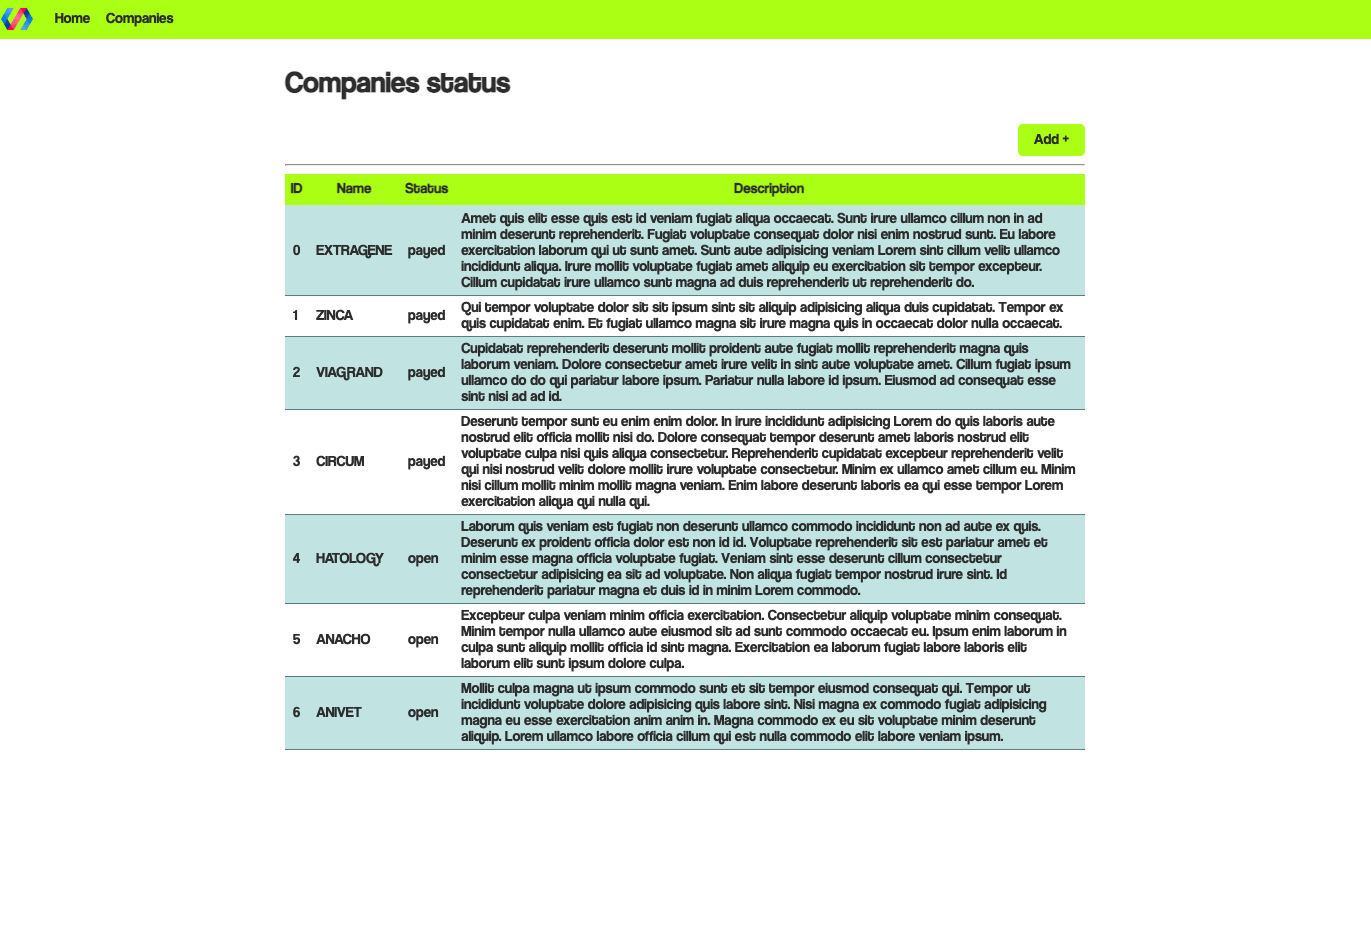
\includegraphics[width=\linewidth, draft=false]{images/demo_view_data_table.png}}
    \caption{Data table page of test applications}
    \label{data_table}
    \end{figure}
The last view (Figure \ref{adding_form}) of the sample applications shows a form for adding new data to the table. The form has three inputs for each value corresponding to the table from the second view. All inputs are simple text inputs with no restriction or validation of the inputs. In a real scenario, there would be validation, but due to the limited time frame of this elaboration, it omits this feature. At the bottom of the form, the user sees a button to save the form. This button is disabled until all input fields are filled have a value. 
\begin{figure}[htbp]
    \centerline{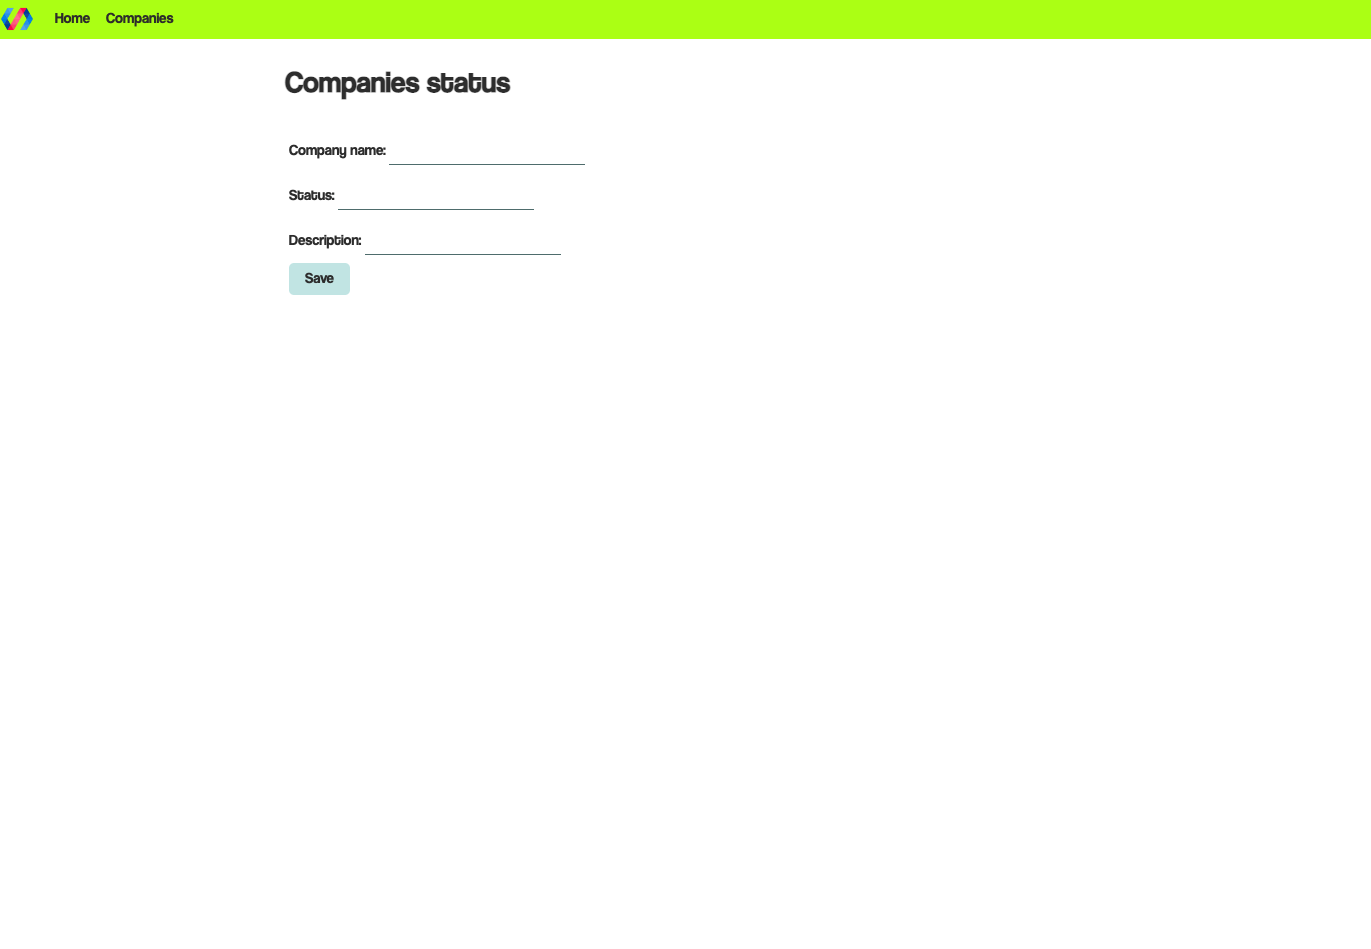
\includegraphics[width=\linewidth, draft=false]{images/demo_view_form.png}}
    \caption{Data adding view of test applications}
    \label{adding_form}
    \end{figure}
\\
Both applications have not only the same views but also the same technology stack. They use Svelte, a library for building web applications with a small package size. According to the starter guide, we use Rollup as a bundling and compilation tool. So both applications do not differ in terms of technology and build steps. \cite{svelte_svelte_nodate} \\
The only difference between the two systems is the implementation details. The following chapters will explain each application's structure and how views are created with and without \ac{SDS}.
\subsubsection{Application using \ac{SDS}}
The first step summarizes how to use the \acl{SDS}. Next, the application must import the code that adds the components from the design system. In this case, the system contains the bundle described in \ref{SDS_build_and_integration}.
The  \texttt{main.ts} file imports the bundle files. Finally, the rollup configuration defines the  \texttt{main.ts} files as an entry files. \\
\lstinputlisting[linerange={1-9},firstnumber=1,caption={Bootstrapping of Svelte application with \ac{SDS}},label=BootstrappingAppSDS]{../Code/sds-demo-app/src/main.ts}
As seen in Listing \ref{BootstrappingAppSDS}, the bootstrapping of the Svelte application is performed here by creating the Svelte App component and appending it to the body. Also, in lines 2 and 3, the SDS bundle Javascript and \ac{CSS} are imported. The import adds the design system components and their styles to the application. Now it is possible to use all the web components within the application via the \ac{HTML} tags defined by \ac{SDS}. \\

After successfully bootstrapping the application, the next step is to look at the Svelte components and how they build the given views. Since the \texttt{App.svelte} component only bootstraps the application and initializes the router, the component does not need further investigation. Therefore, according to the routing details, the next component to be loaded is \texttt{Main.svelte}. \\
The Main component is responsible for displaying the navigation bar, which is visible at the top of each displayed view. In addition, it contains a content placeholder where other components are displayed.  The component's code shows the usage of web components from the  \ac{SDS}. Lines 7-11 in Listing \ref{MainSvelteSDS} use the navigation bar (\texttt{<saas-navbar>}) and the corresponding navigation bar items (\texttt{<saas-navbar-item>}).
\lstinputlisting[linerange={1-14},firstnumber=1,caption={Main.svelte with \ac{SDS}},label=MainSvelteSDS]{../Code/sds-demo-app/src/components/Main.svelte}
The component takes advantage of the functionality of slots by inserting elements into the navbar component. The web component takes care of the corresponding display at the top. The Navbar elements inside ensure that the declared navigation links show up with the correct styles defined by the design system. A special feature in line 8, Listing \ref{MainSvelteSDS} is the \texttt{<img>} element. This \ac{HTML} element is responsible for displaying the logo in the upper left corner. The element has a special property called "slot". Its value is "logo". The web component of the navigation bar recognizes this slot definition and inserts the image with the common styles in the navigation bar. \\
Below the code for the navigation bar, lines 12-14, Listing \ref{MainSvelteSDS}, contain the code for displaying the application's content. In addition to the navigation bar web component, the design system also provides the content component. It uses the same logic as the navigation bar by providing a placeholder for elements within that component and applying styles to the content contained within the web component. Adjustable by design token within the SDS. The \texttt{<Router>} tag within the content is an imported Svelte component that handles the display of the content according to the visited route. \\
For example, one route that is the start of the test is the landing page.The Svelte component \texttt{Home.svelte} represents this page. This component consists only of a few paragraphs and images to distract the user. Therefore, it is not necessary to go into details here. The final result of the view is visible in Figure \ref{landing_page}.\\
An essential component in this comparison is \texttt{Data.svelte}. As the name suggests, this component manages the view of the data table shown in Figure \ref{data_table}. In addition, however, the component's code manages the view of the data table and the view of the data entry form shown in Figure \ref{adding_form}. \\
\lstinputlisting[linerange={84-90},firstnumber=84,caption={Data.svelte with \ac{SDS} table implementation},label=DataSvelteSDSTable]{../Code/sds-demo-app/src/components/Data.svelte}
SDS provides a web component for data tables, visible in in line 89 in Listing \ref{DataSvelteSDSTable}. In order to display the data in the table, two properties are mandatory. 
First, as the name implies, the header property manages the \texttt{header} displayed in the table.  The \texttt{hedaer} object defines a mapping of keys of the table data to the string values that show up as table headers. \texttt{myArray} is the data object handed into the data property of the table web component. Accordingly, the second property is the data input for the table. The data structure of the array should match the data keys defined in the header object so that the data objects within the array match the table headers. \\
Figure \ref{data_table} shows a button at the top of the table. The code snippet also adds the button. Lines 85-87 show the code for the added button. As with the table component, the design system provides a button component thatSection \ref{sds_button} introduced. The \texttt{on:click} property is an indicator of an event listener in Svelte. In this case, a click listener. The event property connects to the \texttt{addEntry} function within the \texttt{Data.svelte} component. This function toggles the boolean variable \texttt{isAddEntry} to \texttt{true}. When the variable changes, the if statement on line 84 is \texttt{false} and activates the else block at line 90. \\

As described in the flow above, the else-block consists of elements to create the view of Figure \ref{adding_form}, the form view. The code snippet looks like this:
\lstinputlisting[linerange={90-100},firstnumber=90,caption={Data.svelte with \ac{SDS} form implementation},label=DemoSvelteSDSForm]{../Code/sds-demo-app/src/components/Data.svelte}
The standard form element between lines 91 and 99 contains the form inputs and a "Save" button. Like the table and the buttons, the form input fields are web components of the design system. The inputs have custom properties for setting the label and its ID to ensure appropriate accessibility. A unique feature of this web component is the custom event for a value change. For example, in line 92, Listing \ref{DemoSvelteSDSForm}, the input receives an event object through this value event and deconstructs the event object to access its details. These details include the changed value of the input field. The newly created data object assigns this value to itself. \\
After all input fields have set a value in the new data object, the "Save" button changes its property \texttt{disbaled} to \texttt{false} and allows click events.Finally, the freshly created object is attached to the data table array with a final click on the button and appears at the bottom. This walkthrough shows all the possibilities of the first test system, and the next section explains the other variant without using the \ac{SDS}. 

\subsubsection{Application not using \ac{SDS}}
One of the main goals is to have a similar application with the same capabilities but not use the design system. So it is necessary to recreate the application from the previous section without using its components. \\
This application uses the same technical stack as the first demo system to avoid significant technical differences between both systems. The bootstrapping of the application looks the same. Listing \ref{MainSvelteSDS} shows it but without the import of SDS code and styles. The application runs and uses Svelte components to create the views described above. \\

As before, a detailed look at the App.svelte is unnecessaryas it is only where the \ac{SPA} initializes the routing. So instead, the first code is in the \texttt{Main.svelte} component to see how this type of application constructs the navigation bar and router content. 
\lstinputlisting[linerange={1-17},firstnumber=1,caption={Main.svelte without \ac{SDS}},label=MainSvelteNormal]{../Code/normal-demo-app/src/components/Main.svelte}
Besides using fewer lines of code compared to Listing \ref{MainSvelteSDS}, the main difference is that no custom web components build the navigation bar or its elements. Here, web standards help by using the correct \ac{HTML} tags to describe specific areas of the application. \\
For example, the navigation bar uses the \texttt{<nav>} tag in lines 6-12 to enclose an unsorted list that tells the browser that this is a navigation area for the application. The same construct of an \ac{HTML} tree was used in the \ac{SDS} demo but hidden behind web components, so the developer does not have to think about it when implementing a navigation bar. \\
The same concept is visible below the navigation bar code in lines 13-17, Listing \ref{MainSvelteNormal}. Here the main content is encapsulated by a \texttt{<main>}, which is also an indicator for the browser. \\
Nevertheless, the part that is not visible in Listing \ref{MainSvelteNormal} and gives the \ac{HTML} element this good look is the styling. Since the \ac{SDS} components are built based on best practices from across the field, no one has to develop a new styling concept and fix style glitches that may occur during development. 
\lstinputlisting[linerange={18-48},firstnumber=18,caption={Main.svelte styles without \ac{SDS}},label=MainSvelteNormalStyles]{../Code/normal-demo-app/src/components/Main.svelte}
As seen in Listing \ref{MainSvelteNormalStyles}, many styles have fixed values for style rules. As in line 23, it is possible to define design tokens in an application and use them in place of the fixed values. However, this usage does not guarantee that the application uses them every time. In an existing design system, components ensure the usage of the defined design tokens. \\
Nevertheless, it is not just consistency that is important. It is also the time required to rewrite those lines of code repeatedly for each new application. Ultimately, this code snippet produces the same view of Figure \ref{landing_page} as in the other demo, but it takes a lot more thinking to get to this result.  \\

The demo project without using the SDS also creates the second view shown in Figure 8, the data table. The project contains a svelte component named \texttt{Data.svelte}, as in the previous section. As in the other application, Data.svelte consists of two views simultaneously. \\
The responsible code snippet looks like this:
\lstinputlisting[linerange={86-92},firstnumber=86,caption={Data.svelte without \ac{SDS} table implementation},label=DataSvelteNormalTable]{../Code/normal-demo-app/src/components/Data.svelte}
At first glance, the component code looks similar to that in Listing \ref{DataSvelteSDSTable}. However, the names of the \texttt{<SvelteTable>} table component and the \texttt{<SvelteButton>} button component hint at of how the application constructs these components. Both Svelte components replicate the logic familiar from the Web components presented earlier. \\
One might ask why it is necessary to build web components when it is possible to build them this way and ensure no style inconsistencies. The answer is that this works for an application with this specific technology stack to reuse these Svelte components. If one is okay with using a limited technology stack to ensure the use of a specific component library, then that is fine. However, the reality is that there are many different frameworks, each with a specific component implementation.\\
In this case, the application builds each component and uses it here, as shown in lines 88 and 91 in Listing \ref{DataSvelteNormalTable}. \\
For example, \texttt{<SvelteButton>} represents the button in the upper right and receives an event to switch to the third view, the form view.Because it is a standalone component, the buttons' styles are not in the \texttt{Data.svelte} component's code but in the button's code. In addition, as explained with the navigation bar, the button styles are defined as fixed values, not as design tokens that a design system would provide. These fixed values cause difficulties when changing the appearance of multiple components with a single value change. \\
The same rules apply to the table component just presented. Therefore, both properties are responsible for ending up in the table in Figure \ref{data_table} as the render result. This explanation sets up the second view and a click on the button reveals the third view (Figure \ref{adding_form}). \\

As the last detail, it is time to look at the code that creates the form for entering a new data object into the table. These elements are visible if the if-statement from line 86, Listing \ref{DataSvelteNormalTable}, results in a \texttt{false} statement, ergo, \texttt{isAddEntry} is \texttt{true}. The result is the block of code that displays the input fields in the browser:
\lstinputlisting[linerange={92-99},firstnumber=92,caption={Data.svelte without \ac{SDS} form implementation},label=DataSvelteNormalForm]{../Code/normal-demo-app/src/components/Data.svelte}
A new svelte component can be seen in lines 94-96, Listing \ref{DataSvelteNormalForm}. As the name \texttt{<SvaleteInput>} indicates, this component is a text input field for the form. However, in addition to the familiar property of indicating an input by specifying a string value, there is a particular Svelte property. The keyword \texttt{bind} indicates a two-way data binding in Svelte. A two-way data binding means the assigned value is available in the component. Therefore, if this variable changes its value within the component, it also reflects the changes outside of it. \\  
Recalling the code snippet from the web component implementation (Listing \ref{DemoSvelteSDSForm})to compare both versions shows it is impossible to \texttt{bind} a value and the event output of a custom web component. In this case, it was necessary to listen to the event manually to get the details. So maybe it is worth avoiding using web components in frameworks because of the lack of such features. \\
With the addition of the button component in line 97, Listing \ref{DataSvelteNormalForm}, the implementation of the form to submit new data to the data field is complete. As with the web component implementation, the button has a \texttt{disabled} property that blocks click events when set to true. Validating the form's input values will either disable the button or not. \\


This last functionality concludes the details of the implementation of the demo systems used to test the SDS. The next step is to examine the test case to test the design system. 
% View 3 
\subsection{Test case}\label{text_case}
A test case helps determine whether a design system created for a common purpose helps users work better with an application. In this elaboration, one test case is performed with two test applications to get better test results. One with \ac{SDS} implemented and one without \ac{SDS}.  \\
Since both systems are visually identical, it is impossible to test them with the same person. The tester would already know how to operate and navigate through the test system by the second run. Therefore, it is necessary to perform a reasonable number of test runs on both systems with approximately the same type of person. By person type in this elaboration is meant what a person does in his daily job, e.g., accountant.  \\
The test provides two results for this elaboration. First is the observation of the test execution for each person. The purpose of this observation is to see how the subject responds to the navigation structure of the web page. How the subject navigates to the next page? Which controls do the users use, whether mouse, keyboard, or other unique controls? Testing is done in person to capture emotions and reactions to the content's appearance and disappearance. At the end of a test run, the subject is asked for additional feedback on the application just tested. With this subjective input, it is possible to assess whether the use of \ac{SDS} affects anything. \\
In addition, the test uses time measurement points in each application. These points provide objective feedback about the time spent on particular views or actions.Furthermore, the applications locate the measurement points in the same place, so comparing both types is possible. In this way, it is feasible to obtain unbiased data for evaluation. \\
In preparation for the test runs, the two applications with and without implementation of the design system are globally available as static web pages. The test person opens one of the two applications and finds a description of the test procedure. The description informs the user that the following application might implement a design system. After the brief introduction, the first view explains the three test steps to the user:

\begin{enumerate}
    \item Navigate to the data table containing the records of different companies.
    \item Find the action to create a new data record.
    \item Fill out the form and submit a new entry.
\end{enumerate}

Since users are not given any instructions on navigating to the data table or with what details to fill in the new record, users are free to explore the demo application. The test steps are intentionally vague to allow users to develop their patterns in their interaction.  \\
After reading all the instructions, the applications will ask the users to start the test by clicking the "Start" button below. This interaction will trigger the first measurement point, which is the start of the demo. \\
The interaction also takes the users to the landing page shown in Figure \ref{landing_page}. On this page, users need to figure out how to navigate to the companies' data table. By scanning the view, they should figure out how to use the navigation bar at the top to navigate to the Companies page. When the user clicks on the navigation bar, they will navigate to the data table view and the second measurement point will be triggered. Again, the memory stores the measured time needed. \\
In the second view (Figure \ref{data_table}), the user sees the data table containing the entries. To add a new entry to the data table, the user must click on the "Add +" button in the upper right corner of this view. With pressing the button, the view changes to the third view (Figure \ref{adding_form}). As with the last view change, the user triggers a new measurement point, and the time data stores it in the memory.  \\ 
In the last view, the user fills in the given form and clicks on "Save" to store the data in the table. The action again triggers and saves a measurement point for the test. When saving the new data unit in the table, the user is navigated back to the table and automatically downloads a JSON file containing all the measurement points described. This JSON file is then sent to the author of this elaboration to collect the measurement of each participant. \\

By collecting all the measurement data and observing the user behavior during the interaction, this test case provides much data for evaluation. These final words conclude this chapter and lead to the next chapter, presenting the test results and their evaluation. 
\subsection{Execution} 
\newpage
\section{Test results}
This chapter presents the results of the test cases performed in Chapter 4. The test was conducted in an enterprise environment. All test participants use SaaS products in their daily work. A total of 22 test runs were performed. These were divided equally between the two test systems. \\
Test candidates try to fill as many different positions as possible. This helps to give a more general meaning to the data obtained. Table \ref{tab:test_candidates} gives an overview of the selected test candidates. \\
\begin{table}[ht]
    \centering
    \begin{tabular}{|p{0.4\linewidth} | p{0.1\linewidth}|p{0.1\linewidth}|}
        \hline
        \textbf{Role} &\textbf{Normal}&\textbf{\ac{SDS}} \\ \hline
        Software Engineer & 7 & 4 \\ \hline
        Cusomer Success & 0 & 2 \\ \hline
        Intern & 1 & 0 \\ \hline
        Consultant & 0 & 1 \\ \hline
        Product Manager & 1 & 0 \\ \hline
        Customer Support & 1 & 0 \\ \hline
        Operation Manager & 0 & 1 \\ \hline
        Engineering Manager & 0 & 1 \\ \hline
        Director Engineering & 0 & 1 \\ \hline
        Customer Success Engineer & 1 & 0 \\ \hline
        IT Support Engineer & 0 & 1 \\ \hline \hline
        \textbf{Total} & 11 & 11 \\ \hline
    \end{tabular}
    \caption{\label{tab:test_candidates} Test candidates}
\end{table}

The list contains various positions from operational and lower management, but also some test candidates from higher management. Unfortunately, the majority of the test candidates are from the software development department, which could be related to the relationships of the author of this elaboration. \\

\subsection{Observation}
As a first step, this elaboration provides the test results of the observation of the test runs. These observations were carried out subjectively and provided information about the test candidates' reactions when dealing with the two systems.\\
Participants took a long time to reach the home page in every other test run. This user behavior shows that the distraction page works well. After the test run, participants indicated in the feedback session that they would move faster if they did not know this was a test. Overall, participants who took a long time on the home page stopped reading and immediately scrolled to the top of the page to get to the data table. There were no differences in interaction between the SDS testing system and the regular system. \\
As with the long distraction, participants show a pattern of quickly finding the "Add +" button to add a new entry in both applications. As with the long distraction, participants show the pattern of quickly finding the "Add" button in both applications to add a new entry. Then, participants continue adding data to the form without responding to the second view. Observation shows that there is one more entry in the normal application than in the \ac{SDS} application, which the test user cycled through the test application quickly. However, the notes show they were relatively even in their cycle time.  \\
Summarizing the observations when adding the data to the table, it seems that entering the data into the normal system was faster. Users quickly enter the data into the form and submit the form immediately. Furthermore, none of the participants ever asked for values for the status because the field was left open as a text box instead of offering a drop-down list. In comparison, two participants in the \ac{SDS} implementation application ask for preset values for status on the form. Of course, the selecting participants could also relate to this phenomenon.  \\
All in all, the observations of the test runs show no decisive differences between the two systems. However, one interaction that stood out in both applications was the tryout pattern instead of reading through the text or navigation bar elements. Instead, the user tried clicking on every element, resulting in a quick run through the test application but showing that \ac{SaaS} products should be intuitive. 

\subsection{Measurements}
This chapter presents the insights from the measurements taken during the test runs. These measurements can confirm the subjective observations made earlier. With the help of the measurement points presented in Chapter \ref{text_case}, it is possible to analyze the data collected. For example, if we take the duration between two measurement points, we obtain three timeslots. 
\begin{enumerate}
    \item \textbf{Find data table}: Starting the test - see the data table
    \item \textbf{Find add button}: See data table - see data add form
    \item \textbf{Add data to table}: See data add forme - submit data add form
\end{enumerate}
With the help of the measurements, it is possible to draw diagrams to understand the collected data better. One problem encountered when looking at the data is that the total duration of each run varies from run to run. A transformation with the collected data ensures that all results are comparable. In detail, the transformation calculates each duration slot relative to the total duration. All sections together result in a total percentage of 100\%. \\

With the prerequisites explained, it is time to look at the data. Starting with the measurements of the test runs on the application without \ac{SDS}.\\

\begin{figure}[htbp]
    \centerline{
    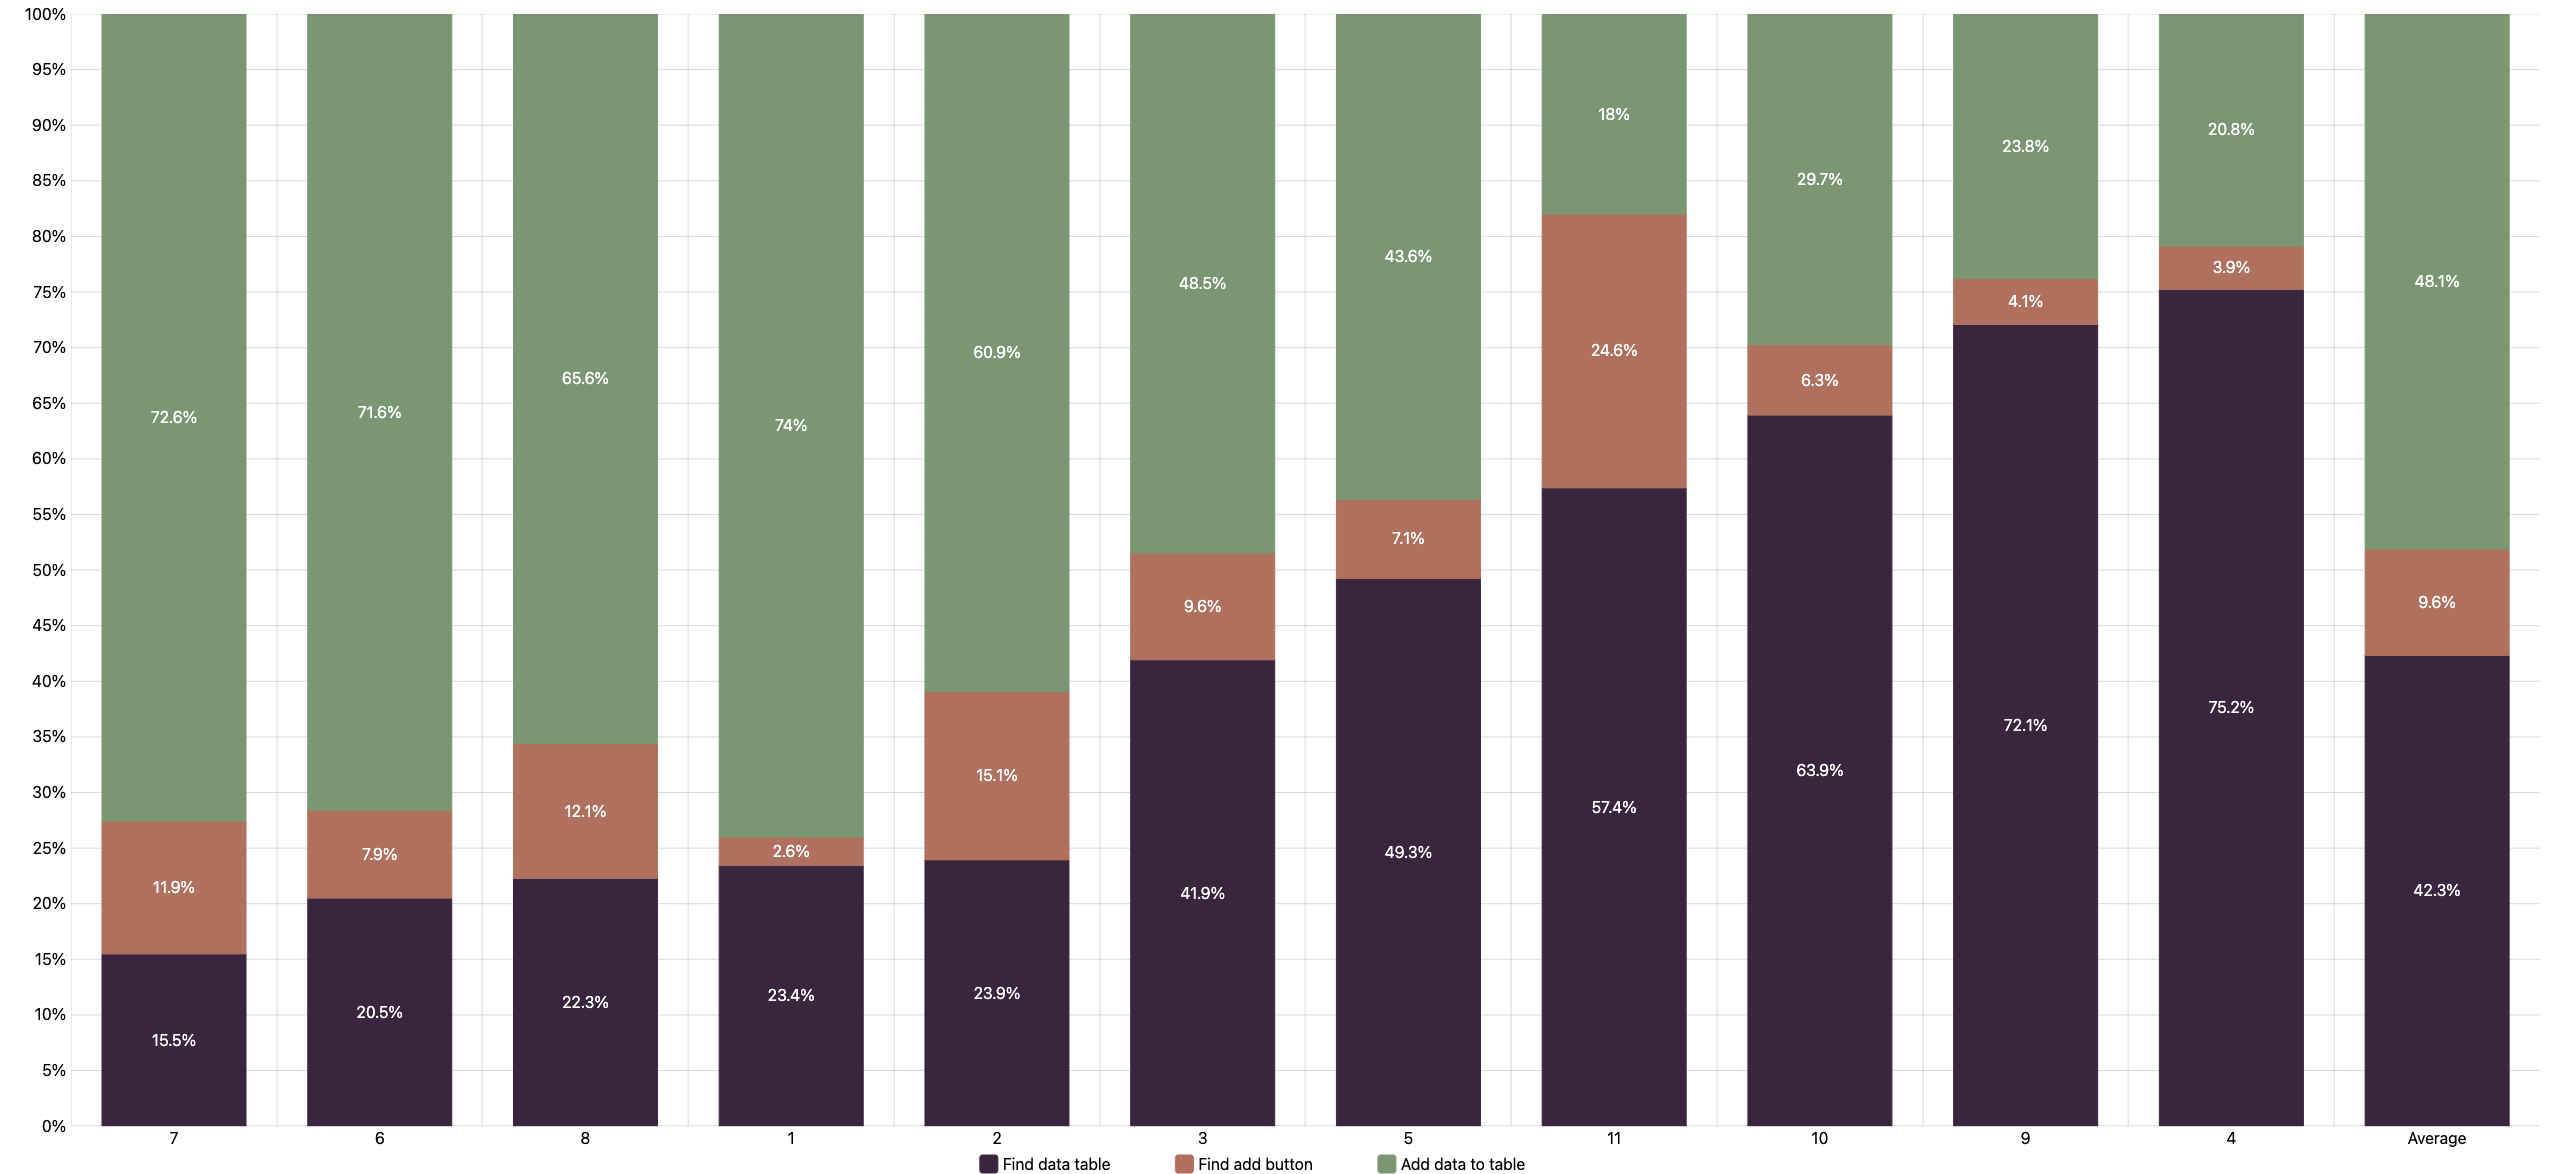
\includegraphics[width=\linewidth]{images/normal_test_data_chart.png}}
\caption{Chart of normal test data}
\label{test_data_normal}
\end{figure}
The chart in Figure \ref{test_data_normal} shows that the data confirms the point made in the observations. Sorted by time to find the data table, the chart shows the distribution of time needed. The first five columns show runs that the users completed test runs very quickly. As a result, data entry takes a relatively long time since typing slows down the user. A look at the end of the chart shows the long runs with a longer time on the home page. \\
The last column of the chart shows the average of all datasets combined. Once again, it is essantial to note that the average time spent on the distribution of finding the data table and adding data through the form is about the same. \\
The only breakout from the schema is the test run 11. In this run, the relative number shows that finding the "Add +" button, i.e., showing the data table, took longer than adding the data. A look at the data shows that this was one of the longer test runs of the data set, lasting almost two minutes. The long time taken indicates that the test user either interacted cautiously with the test application or had trouble navigating. \\
The data chart concludes that there are no surprises in the test runs for the application without SDS. It generally confirms the previously reported observation.\\

As a next step, the elaboration deals with the results of the test run of the application with implemented SDS. Expecting to see roughly the same distribution pattern of test data.  As in Figure \ref{test_data_normal}, this chart shows the relative time windows calculated using the total time required for each run. \\

\begin{figure}[htbp]
    \centerline{
    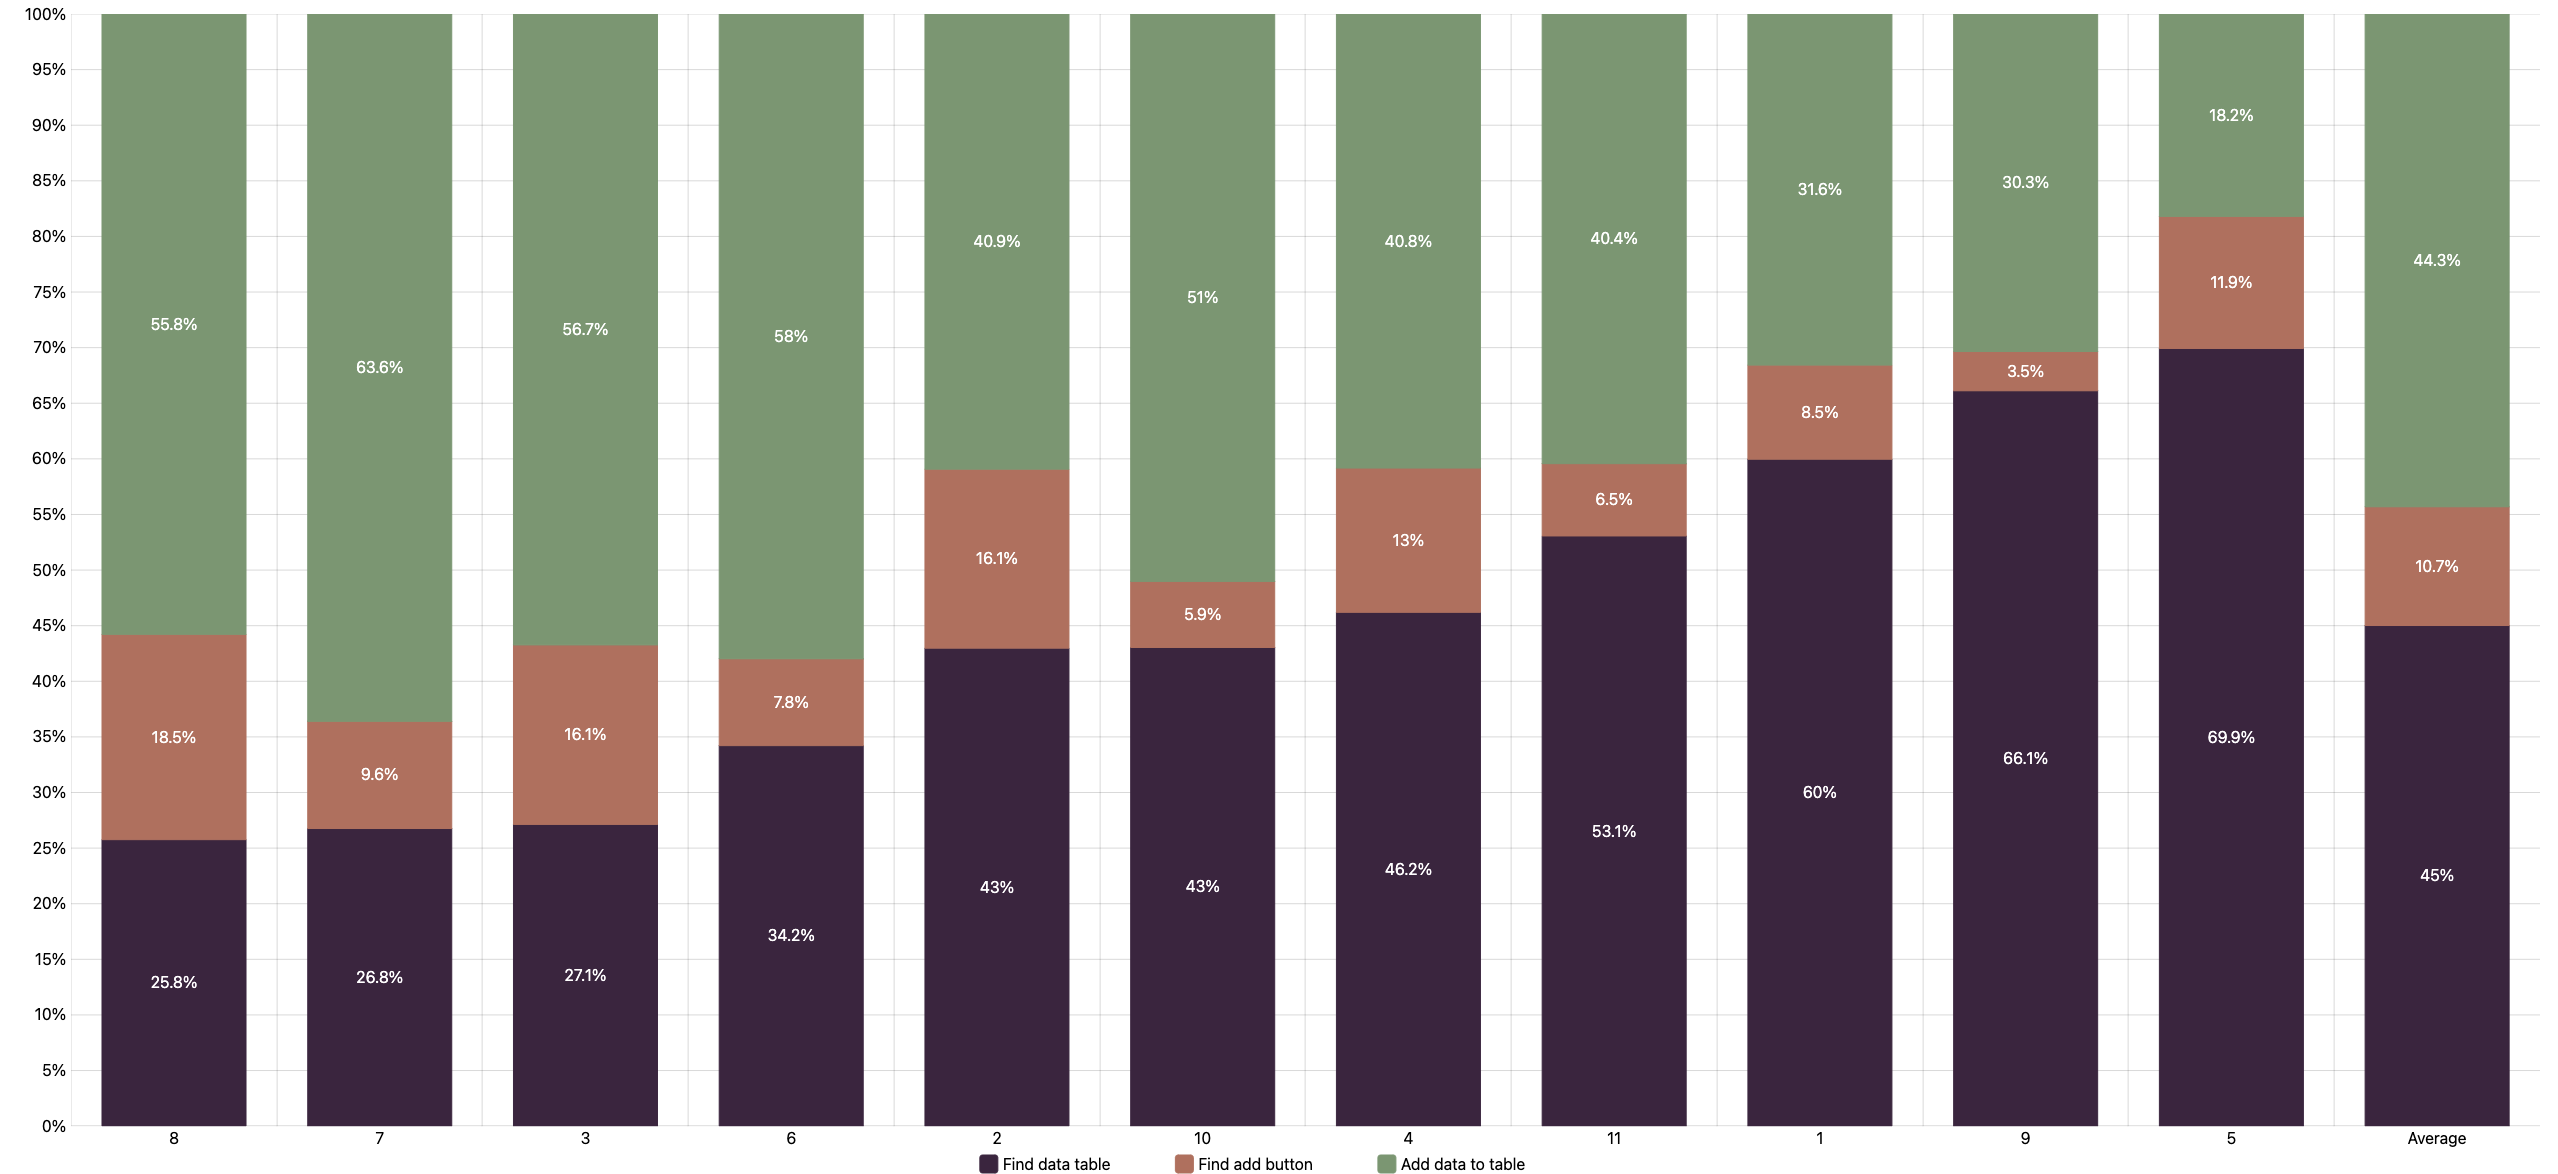
\includegraphics[width=\linewidth]{images/sds_test_data_chart.png}}
\caption{Chart of \ac{SDS} test data}
\label{test_data_sds}
\end{figure}
At first glance, Figure \ref{test_data_sds} shows the same pattern as the normal test data chart. But in closer comparison to the normal data chart (Figure \ref{test_data_normal}), the distribution of the datasets is smoother. This pattern indicates a more even distribution of the time spent on the different time windows. \\
The average column at the end of the chart shows roughly the same distribution of values as the normal data. This similarity means that finding the table of data takes, on average, the same amount of time as entering data into the form. So on average, there is no difference in the test application without \ac{SDS}. \\
As previously seen on the test sets, no runs indicate a breakout. The only interesting thing is that the search time for the "Add +" button in three test runs accounted for over 15\% of the total time. A look at test runs 8, 3, and 2 in Figure \ref{test_data_sds} shows that these tests are short overall. Therefore, a 4-second mouse movement on the button ends in a distribution of 15\% if the entire run takes only 30 seconds. However, this is not unusual user behavior in the test application.\\
Summarizing the analysis of the data chart from the test runs of SDS data, the chart shows a smoother curve which could indicate a broader group of test users. Because every user has a different interaction approach when using a tool. The chart shows the same usage patterns as in the normal test data.  \\

In order to obtain comparable test data within the test sets, it was necessary to draw a boxplot diagram. The boxplot diagram collects the total duration of each test run in one diagram. This diagram helps compare the two test sets based on the median, maximum, minimum, lower quartile, and upper quartile. \\

\begin{figure}[htbp]
    \centerline{
    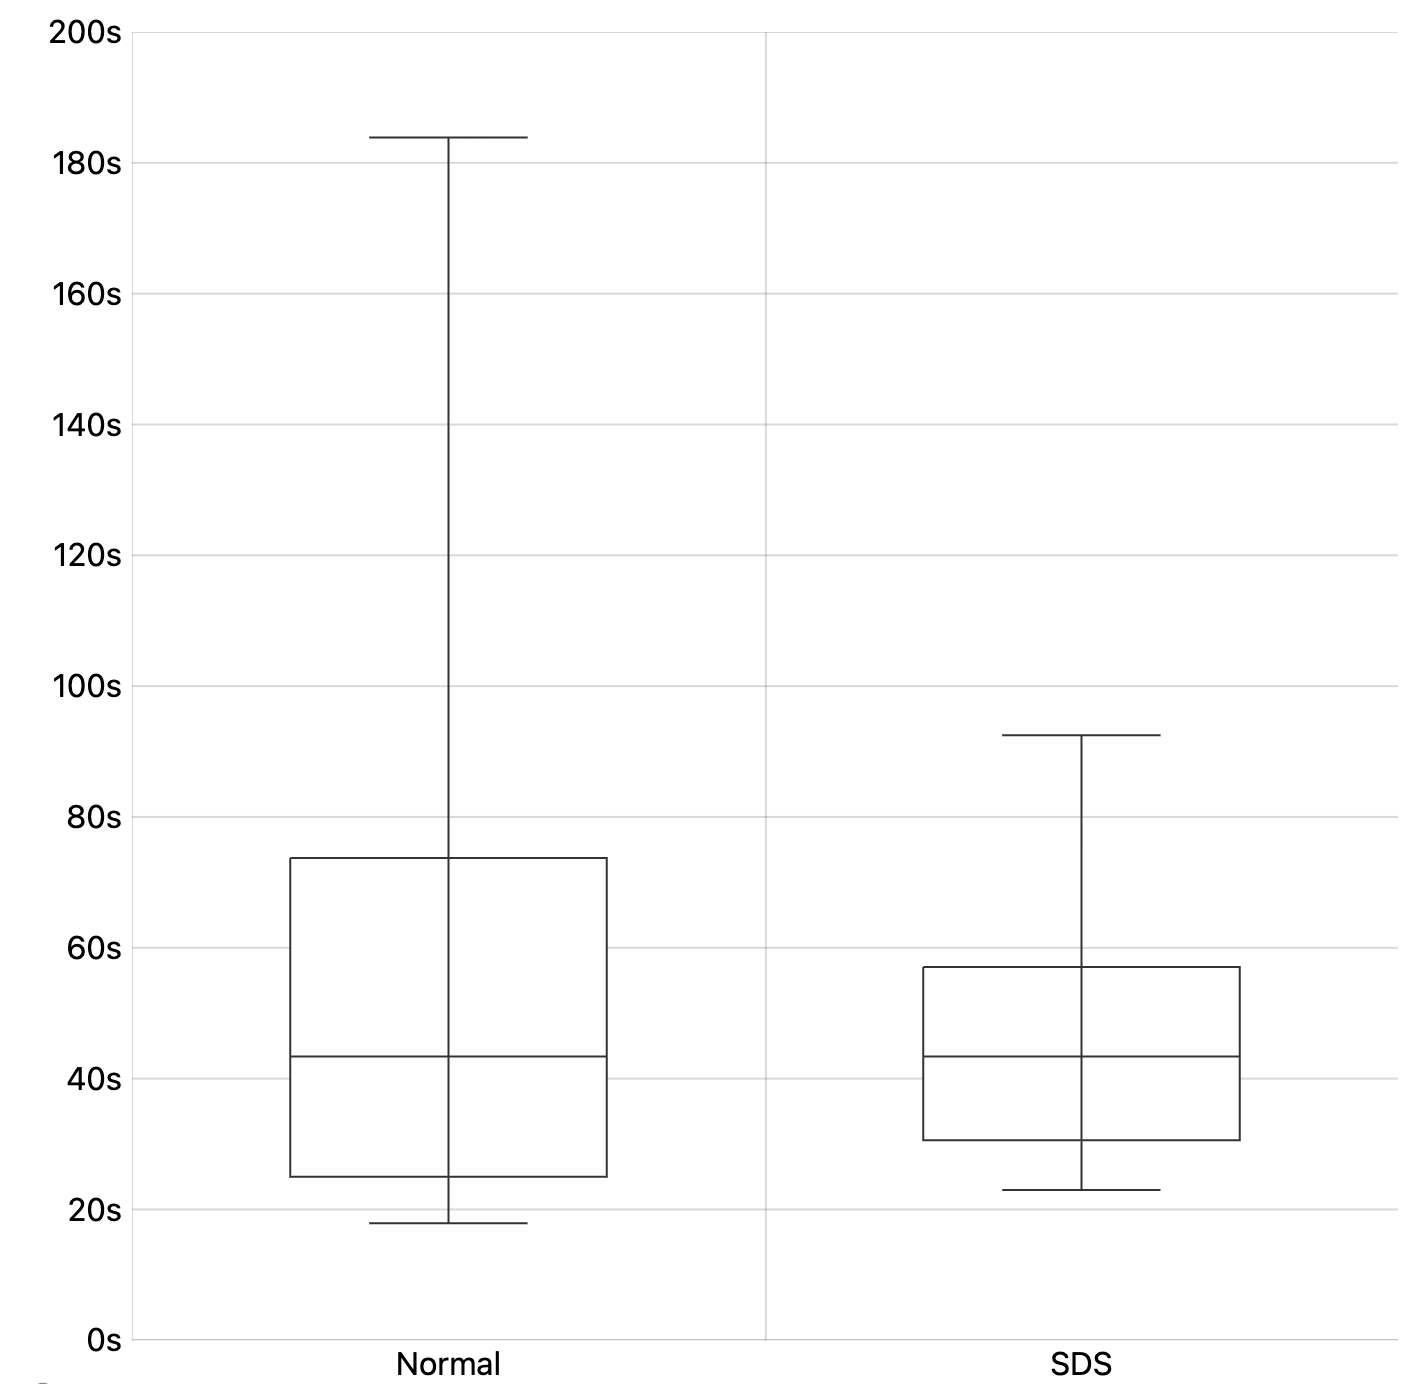
\includegraphics[height=10cm]{images/box_plot_total_duration.png}}
\caption{Boxplot diagram for comparison of both test sets based on the total duration}
\label{box_plot_comparison}
\end{figure}
Figure \ref{box_plot_comparison} shows both test sets in a boxplot diagram. The y-axis describes the total time required for the test runs in seconds. On the other Axes, the x-axis shows both test runs, the normal test run without \ac{SDS} and the test run with \ac{SDS}. \\
First, consider the two boxes in this diagram. The box for the normal test runs is larger overall than for the \ac{SDS} tests. This difference means that the runs with \ac{SDS} are closer than those without \ac{SDS}. As for the numbers, the normal test data is in the lower range of the box. The lower quartile is 24 seconds for the normal data. \\
In comparison, the \ac{SDS} box starts at 30 seconds. The end of the box for the normal test run is at 73 seconds. The \ac{SDS} box ends at 57 seconds, as explained above. It follows that 50\% of the test runs from the normal data set are between 24 and 73 seconds and correspondingly between 30 and 57 seconds for \ac{SDS}.  \\
The median shows the mean value of the test runs. The diagram represents the median with the horizontal lines inside the boxes. The values for both test runs are precisely 43 seconds. There is only a difference of 300ms. Such a tiny difference shows that the test sets do not differ in this case. \\
The last thing the chart shows are the breakdowns of each data set, represented by the vertical lines that branch off the boxes. At first glance, there is a big difference between the two data sets with the long line on one box. In the case of the normal data set, the breakouts go beyond 180 seconds. This outburst is twice as large as the highest outburst of \ac{SDS} (90 seconds). In turn, the lower bursts are not that different from the 50\% majority represented by the boxes. In both sets of tests, they look pretty similar in size. The only difference visible here is the actual value. For the normal test set, the lowest value of the test set is 17 seconds. For \ac{SDS}, this value is slightly higher at 22 seconds. Nevertheless, a difference of 5 seconds. \\
To sum it up, the chart shows a much greater variety in the test series than in the normal run. However, it also shows that the application without SDS allows users to complete their tasks faster in extreme cases but sometimes much slower. 
\subsection{Test evaluation}
The design of the tests proves the hypothesis of whether the SDS helps users complete a simple task faster than an application without \ac{SDS} implementation. After both test results presentations, it is possible to interpret the results. On the one hand, the subjective observation of each test run and, on the other hand, objective data from performance time stamps during the execution of each test run.  \\
From an observational perspective, it looks like the systems behave pretty similarly. As the results show, there are no particular patterns in either application. The observation indicates that it makes no difference with which application the user performs the task.  \\
The performance data from the test runs show a relatively similar result. In the normal test runs, there seems to be a clear division of usage patterns. For example, a user spends a relatively large amount of time finding the data table or a relatively large amount of time adding data. Compared to the \ac{SDS} test runs, the time patterns are more balanced, with a smooth transition between a long time for finding the data table and a long time for data entry. This pattern difference indicates more extremes in the runs for the normal version.  \\
In addition to this information, the boxplot diagram provides further insights. Again, the noticeable pattern in the normal test runs is visible. TThe normal data has a broader range in the boxplot than the \ac{SDS} test runs. The normal application seems to have a more random interaction pattern than the \ac{SDS} application. However, this is not all bad. The normal data run also better in terms of minimum time. The \ac{SDS} seems to help the application create a more consistent user usage pattern.  \\
In conclusion, using the \ac{SDS} helps to perform tasks more consistently and thus faster. Furthermore, the graph results show that the \ac{SDS} is generally faster. As a final step, the chi-square test evaluates whether the data points presented are statistically significant. \\

The chi-square test, according to \citeauthor{pearson_x_1900}, helps to identify whether an application is faster with \ac{SDS} than without \ac{SDS}. As the first step, a null hypothesis must be defined. In this case, the null hypothesis is whether the application with SDS implemented is faster than the normal application. The result should be significant, with a probability of 95\%. \cite{pearson_x_1900} \\ 
Since it is impossible to compare the data of each set of tests because different users performed them, a different measurement is required. Therefore, the test looks at each run and whether the required time is less than 60 seconds. Summing up the results, the table looks like this:
\begin{table}[ht]
    \centering
    \begin{tabular}{|p{0.2\linewidth} || p{0.1\linewidth}|p{0.1\linewidth}|p{0.1\linewidth}|}
        \hline
        \textbf{Total time under 60 seconds?} &\textbf{Normal}&\textbf{\ac{SDS}}&\textbf{Total} \\ \hline\hline
        \textbf{yes} & 7 & 8 & 15 \\ \hline
        \textbf{no} & 4 & 3 & 7 \\ \hline
        \textbf{Total} & 11 & 11 & 22 \\ \hline
    \end{tabular}
    \caption{\label{tab:chi-square} Aggregated test results}
\end{table}
The next step is to calculate the expected values for each variant. First, the test multiplies each test set by the sum of the results for the met criteria of both runs. Then the sum of all test runs divides the product from before. After processing all values in the table with this method, the table looks like this: 
\begin{table}[ht]
    \centering
    \begin{tabular}{|p{0.2\linewidth} || p{0.1\linewidth}|p{0.1\linewidth}|p{0.1\linewidth}|}
        \hline
        \textbf{Total time under 60 seconds?} &\textbf{Normal}&\textbf{\ac{SDS}}&\textbf{Total} \\ \hline\hline
        \textbf{yes} & 7.5 & 7.5 & 15 \\ \hline
        \textbf{no} & 3.5 & 3.5 & 7 \\ \hline
        \textbf{Total} & 11 & 11 & 22 \\ \hline
    \end{tabular}
    \caption{\label{tab:chi-square-expected} Expected test results}
\end{table}
With the expected and actual values, it is now possible to calculate the chi-square value for each entry in the table. The following formula calculates the chi-square value for each entry:
\[\chi^2=\frac{(A_{jk} - E_{jk})^2}{E_{jk}}\]

$A_{jk}$ is an entry of the actual values table, and $E_{jk}$ is a value of the expected value table. The result is a new table with all $\chi^2$ values. The table looks like this:

\begin{table}[ht]
    \centering
    \begin{tabular}{|p{0.2\linewidth} || p{0.1\linewidth}|p{0.1\linewidth}|p{0.1\linewidth}|}
        \hline
        \textbf{Total time under 60 seconds?} &\textbf{Normal}&\textbf{\ac{SDS}}&\textbf{Total} \\ \hline\hline
        \textbf{yes} & 0.03 & 0.03 & 0.06 \\ \hline
        \textbf{no} & 0.07 & 0.07 & 0.14 \\ \hline
        \textbf{Total} & 0.1 & 0.1 & 0.2 \\ \hline
    \end{tabular}
    \caption{\label{tab:chi-square-results} Chi-squared results}
\end{table}
The total $\chi^2$ value of the test data is \texttt{0.2}. The chi-square distribution table determines the degree of freedom of the table and the specified probability of the value for the statistical relevance. For this test, the value to achieve is \texttt{3.84}. Since the total value is less than the determined value, no statistically significant relationship exists between using the SDS and the total time required to complete the task. \\

Thus, the test results provide a clear statement. While the test results indicate that a design system contributes to consistency in the use of an application, the evaluation of this data concludes that the results are not statistically significant and that the SDS does not affect the performance of completing tasks in an application.
\subsection{Discussion}
 
\newpage
\section{Conclusion}
This elaboration presents a possibility to perform standardization in a different way. A design system represents a way of creating user interfaces for ergonomically correct views. With today's technology and standardized browsers, it is not a problem anymore to find a central solution that allows developers to create reusable components without the application restricting to a certain framework. \\
Chapter \ref{saas_design_system} presents a possible concept for implementing a design system. The \acl{SDS} allows developers and designers to focus more on delivering value to their users because they don't have to worry about accessibility or best practices. The onboarding time for creators is short because a design system provides enough tools to get them started quickly. \\
With all the tools in hand, developers can even build their own design system based on the \ac{SDS}. It gives them a blueprint for a design system. Not only does it extend components through the interfaces provided, but it also gives developers the ability to manipulate the existing components. This leaves enough room for creativity for the own \ac{SaaS} products and their brand.\\
A key feature of the \ac{SDS} is the community aspect that surrounds it. Without it, the \ac{SDS} could be just another component library. But providing principles, guidelines, and a platform for designers and developers is what makes \ac{SDS} special. These community-built values reflect the needs of developers and designers much better than an ISO standard that is updated every two years. In a fast-paced world, a quick response time is important.\\
The results of the test of the \ac{SDS} in Chapter \ref{test_results} show a clear result. Efficiency for the users of \ac{SaaS} products is the crucial point when developing a design system like \ac{SDS}. The test result shows that a design system helps to maintain the consistency of an application. Both test applications are visually designed in the same way. Even though the observation seems to show no difference between the two applications, the data collected shows a different pattern. The test shows that users were able to complete their tasks 20\% faster with the \ac{SDS} application. \\
In summary, the \ac{SDS} is a valid concept for a different kind of user interface standardization for \ac{SaaS} products. Not only is it much easier to implement in existing systems, but it also provides added value for end users. Of course, this elaboration is just a concept of what such a system could look like, and much more work is needed in the real world to create a fully functional system. However, as a first proposal, it might be interesting to follow up on these results.
\subsection{Outlook} 

% choose your type of citation here
%\bibliographystyle{plainnat} % author and year
%\bibliographystyle{amsalpha} % author and year short
%\bibliographystyle{alphaabbr} % author short and year
%\bibliographystyle{alpha} % author and year
%\bibliographystyle{plain} % only numbers
%\bibliographystyle{unibonn_ay} % a special file used for the uni bonn


\newpage
\singlespacing % bibliography with single spacing 
\printbibliography

%% Start of the appendix
\appendix 
%% The appendix is a chapter
\section*{Appendix}
\begin{sidewaysfigure}[tp]
    \centerline{
    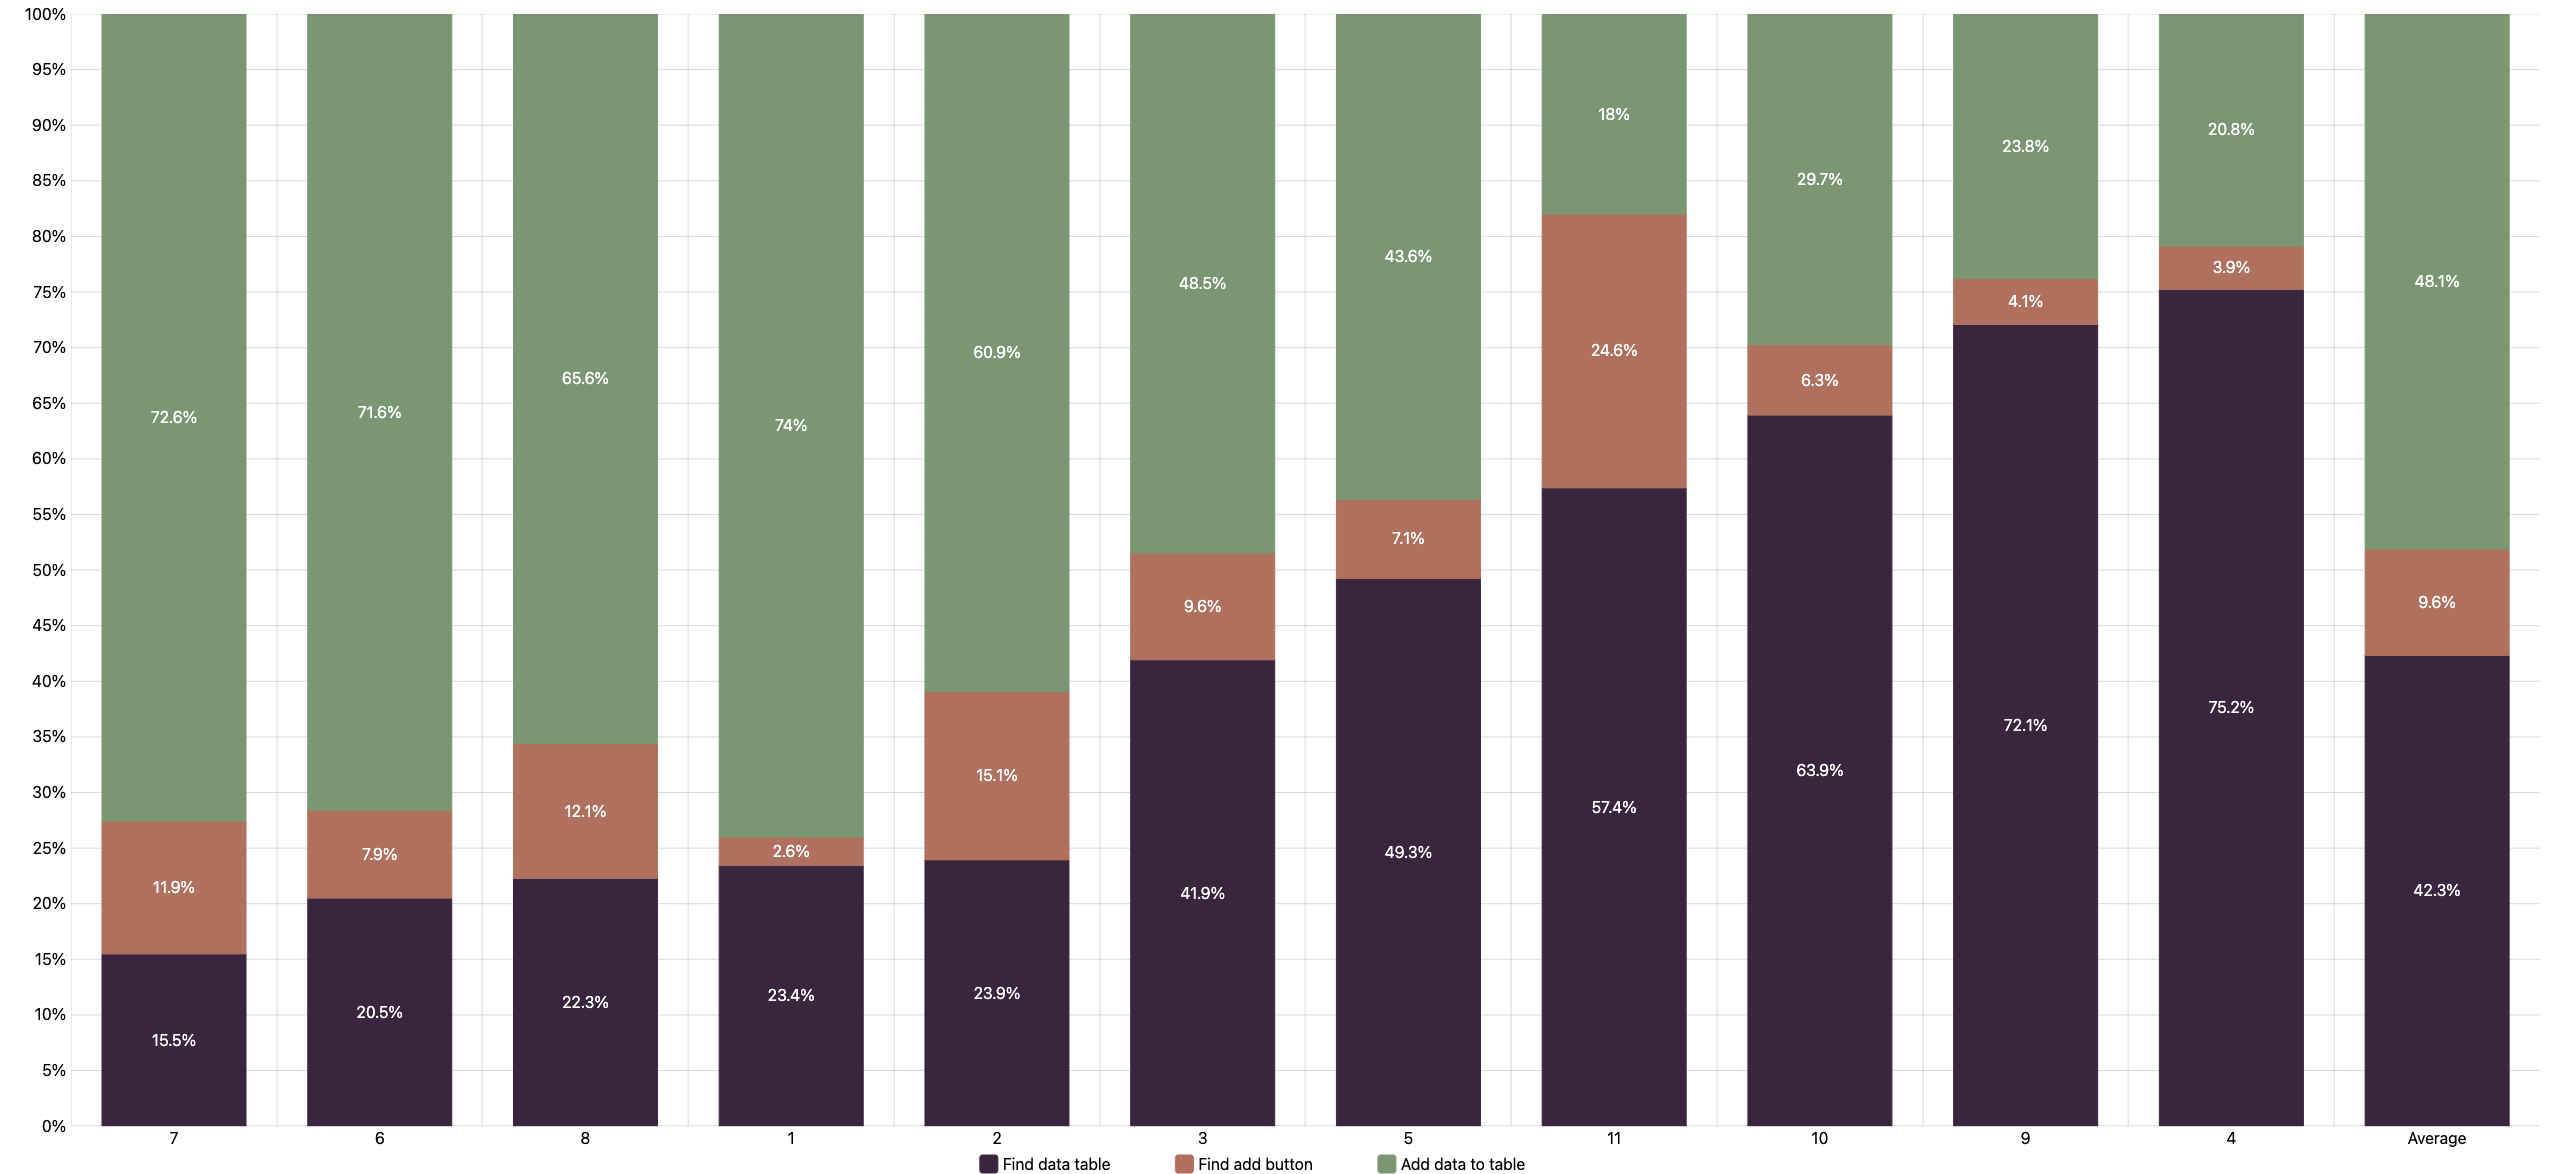
\includegraphics[height=8cm]{images/normal_test_data_chart.png}}
\caption{Chart of normal test data}
\end{sidewaysfigure}
\begin{sidewaysfigure}[tp]
    \centerline{
    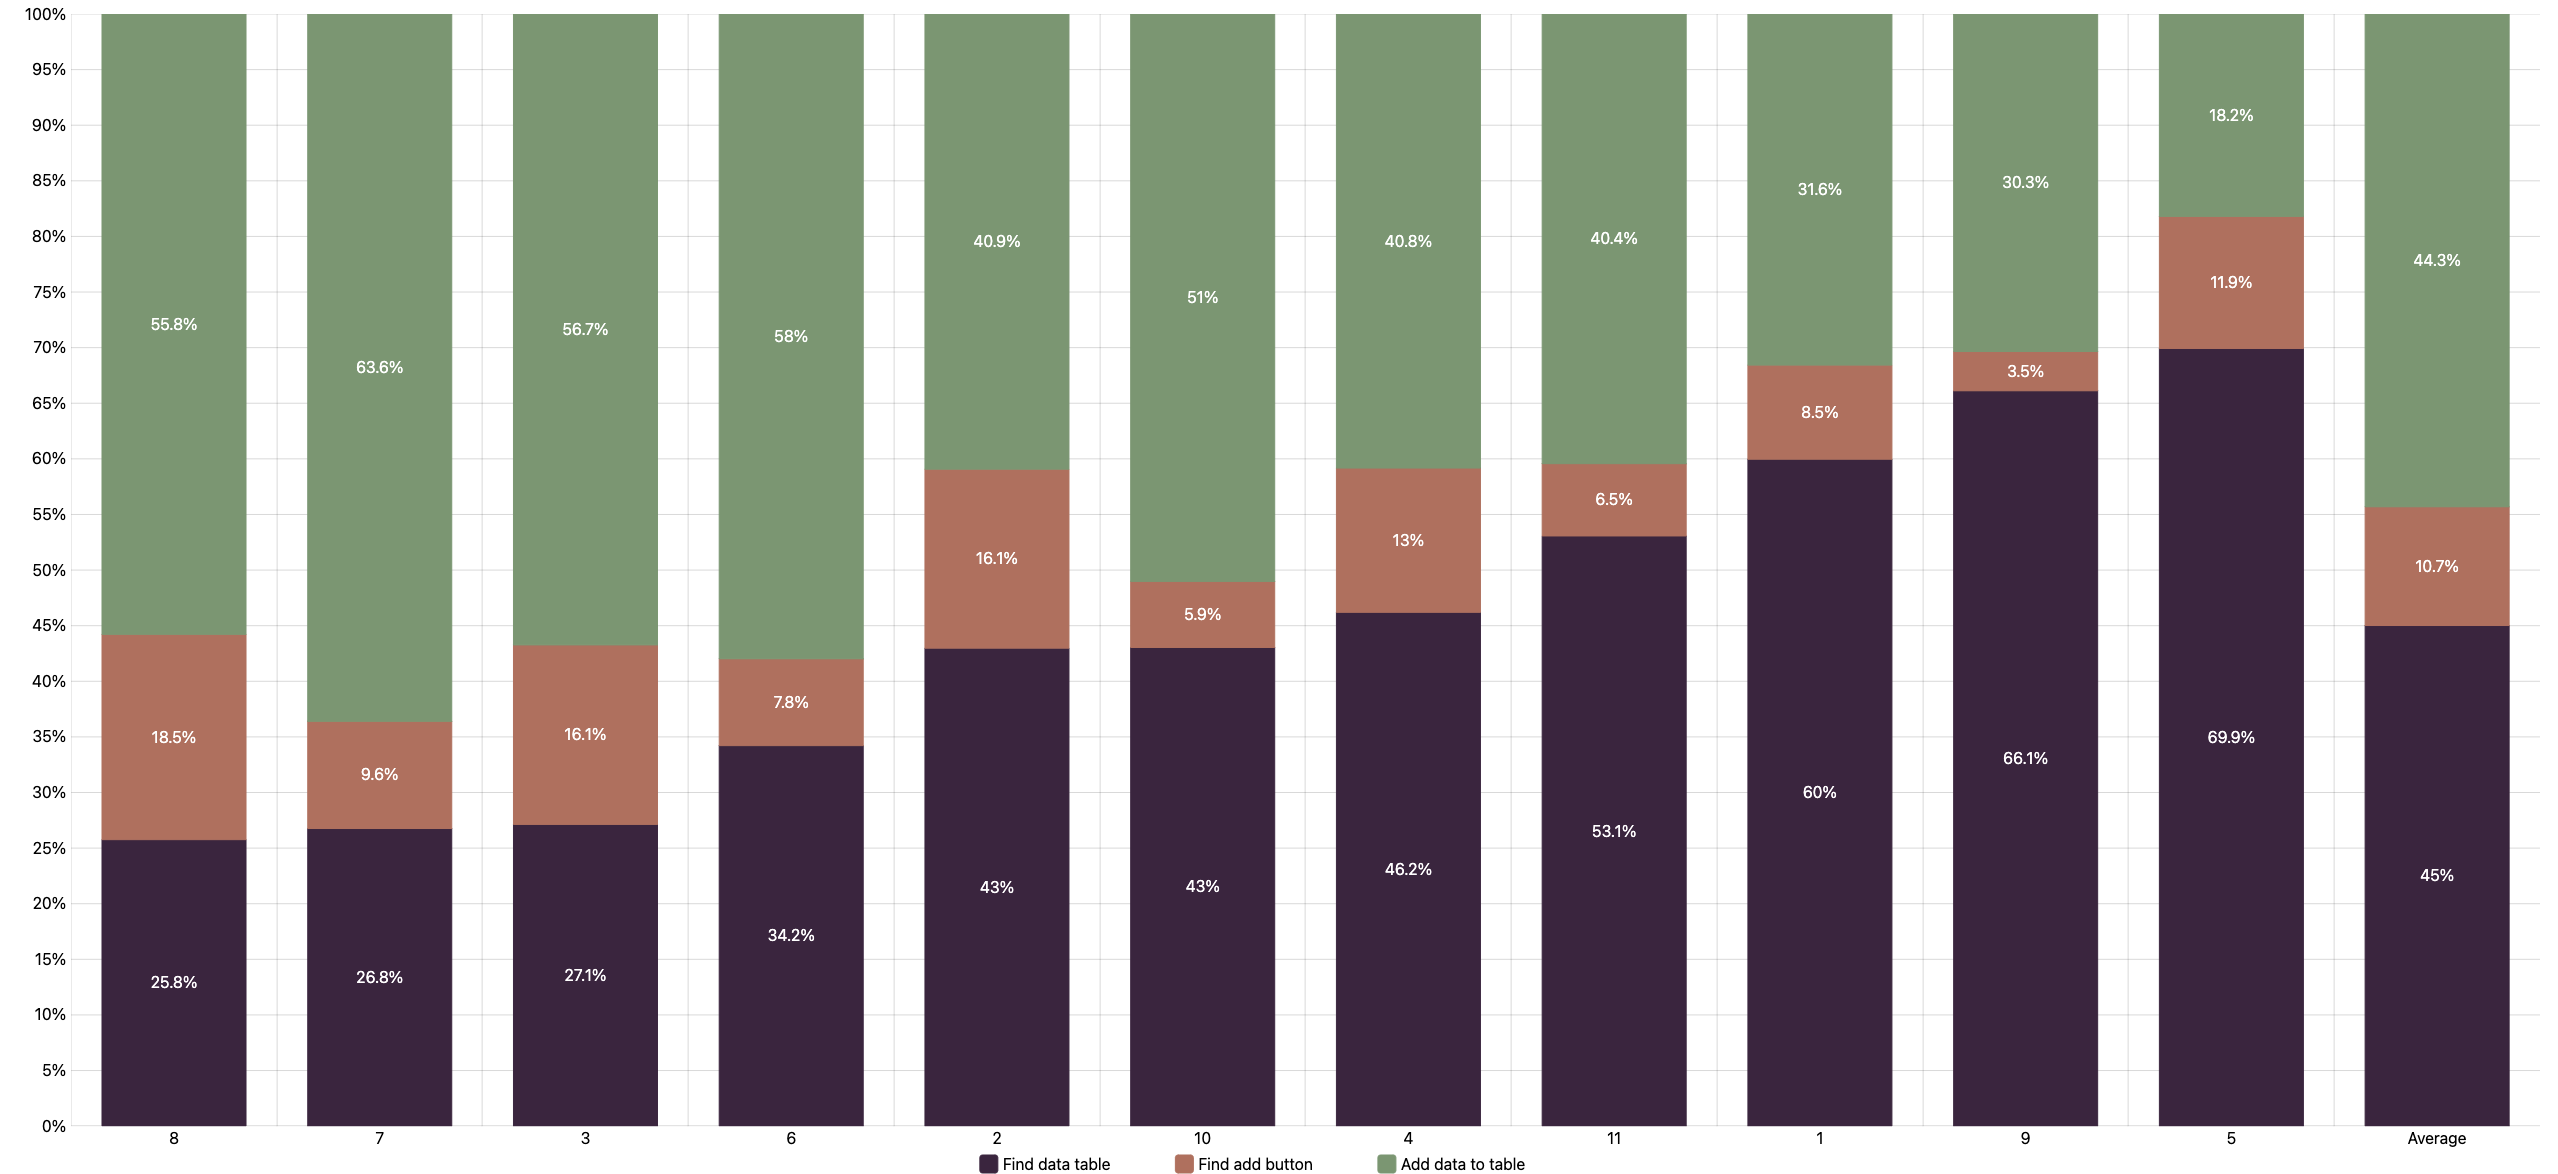
\includegraphics[height=8cm]{images/sds_test_data_chart.png}}
\caption{Chart of \ac{SDS} test data}
\end{sidewaysfigure}

\end{document}
 
